\documentclass[nofootinbib,notitlepage,11pt]{revtex4-2}

%%% linking references
\usepackage{hyperref}
\hypersetup{
  breaklinks=true,
  colorlinks=true,
  linkcolor=blue,
  filecolor=magenta,
  urlcolor=cyan,
}

%%% header / footer
\usepackage{fancyhdr} % easier header and footer management
\pagestyle{fancy} % page formatting style
\fancyhf{} % clear all header and footer text
\renewcommand{\headrulewidth}{0pt} % remove horizontal line in header
\usepackage{lastpage} % for referencing last page
\cfoot{\thepage~of \pageref{LastPage}} % "x of y" page labeling

%%% symbols, notations, etc.
\usepackage{physics,braket,bm,amssymb} % physics and math
\renewcommand{\t}{\text} % text in math mode
\newcommand{\f}[2]{\dfrac{#1}{#2}} % shorthand for fractions
\newcommand{\p}[1]{\left(#1\right)} % parenthesis
\renewcommand{\sp}[1]{\left[#1\right]} % square parenthesis
\newcommand{\spp}[1]{\sp{\sp{#1}}} % double square parenthesis
\renewcommand{\set}[1]{\left\{#1\right\}} % curly parenthesis
\newcommand{\bk}{\Braket} % shorthand for braket notation

\renewcommand{\c}{\cdot} % inner product
\newcommand{\m}{\bm} % bold symbol
\renewcommand{\v}{\vec} % arrow vector

\usepackage{dsfont} % for identity operator
\newcommand{\1}{\mathds{1}}

\newcommand{\up}{\uparrow}
\newcommand{\dn}{\downarrow}

\renewcommand{\i}{\mathrm{i}\mkern1mu}
\renewcommand{\d}{\text{d}}
\newcommand{\x}{\text{x}}
\newcommand{\y}{\text{y}}
\newcommand{\z}{\text{z}}

\newcommand{\A}{\mathcal{A}}
\newcommand{\B}{\mathcal{B}}
\newcommand{\C}{\mathcal{C}}
\newcommand{\D}{\mathcal{D}}
\newcommand{\E}{\mathcal{E}}
\newcommand{\G}{\mathcal{G}}
\renewcommand{\H}{\mathcal{H}}
\newcommand{\I}{\mathcal{I}}
\renewcommand{\L}{\mathcal{L}}
\newcommand{\M}{\mathcal{M}}
\newcommand{\N}{\mathcal{N}}
\renewcommand{\O}{\mathcal{O}}
\renewcommand{\P}{\mathcal{P}}
\newcommand{\Q}{\mathcal{Q}}
\renewcommand{\S}{\mathcal{S}}
\newcommand{\T}{\mathcal{T}}

\newcommand{\PP}{\mathbb{P}}
\renewcommand{\SS}{\mathbb{S}}
\newcommand{\TT}{\mathbb{T}}
\newcommand{\ZZ}{\mathbb{Z}}

\newcommand{\PS}{\text{PS}}
\newcommand{\EQPS}{=_{\text{PS}}}

\newcommand{\oper}{\operatorname}

\usepackage{accents} % for the undertilde
\newcommand{\ut}{\undertilde}
\newcommand{\ot}{\widetilde}
\newcommand{\col}{\underline}
\newcommand{\mean}{\overline}

\newcommand{\lra}{\leftrightarrow}
\newcommand{\floor}[1]{\lfloor{#1}\rfloor}

\usepackage[inline]{enumitem} % in-line lists and \setlist{} (below)
\setlist[enumerate,1]{label={(\roman*)}} % default in-line numbering
\setlist{nolistsep} % more compact spacing between environments

%%% figures
\usepackage{graphicx} % for figures
\graphicspath{{./figures/}} % set path for all figures
\usepackage[export]{adjustbox} % for vertical alignment in math
\newcommand{\diagram}[1]
{\,\includegraphics[valign=c]{diagrams/#1.pdf}\,}

% alphanumeric footnotes
\renewcommand*{\thefootnote}{\alph{footnote}}

% for energy diagrams, etc.
\usepackage{tikz}
\usetikzlibrary{arrows,math,calc}
\tikzstyle{every picture}+=[remember picture]
\tikzset{
    thickest/.style={line width=3pt}
}

%%% text markup
\usepackage{color} % text color
\newcommand{\red}[1]{{\color{red} #1}}

%%%%%%%%%%%%%%%%%%%%%%%%%%%%%%%%%%%%%%%%%%%%%%%%%%%%%%%%%%%%%%%%%%%%%%
\begin{document}

% todo: solve collective model; Casmir operators?

\title{SU($n$) ferromagnets near the Heisenberg critical point}%
\author{Michael A. Perlin}%
\date{\today}

\maketitle

\tableofcontents

\section{Introduction}

SU($n$) symmetries play an important role in physics.  Underpinning
much of high energy physics, the celebrated SU($n$) gauge theory known
as Yang-Mills theory is central to our understanding of the
electroweak and strong forces.  Extensions of Yang-Mills and SU($n$)
symmetry feature in the most well-studied examples of holographic
duality\cite{maldacena1999largen} and the connection between
entanglement and gravity\cite{ryu2006holographic} through the anti-de
Sitter / conformal field theory (AdS/CFT) correspondence.  In a
condensed matter setting, SU(2) appears ubiquitously as a symmetry of
the Hubbard model, with important consequences for the study of
quantum magnetism and high temperature
superconductivity\cite{lee2006doping}.  The extension of the SU(2)
Hubbard model to SU($n$) has led to predictions of exotic phases of
matter such as valence bond solids\cite{read1989valencebond,
  rokhsar1990quadratic, kaul2012lattice, hermele2011topological} and
chiral spin liquids\cite{hermele2009mott, hermele2011topological,
  chen2016syntheticgaugefield, nataf2016chiral}, as well as the
potential to perform universal topological quantum
computation\cite{freedman2004class, nayak2008nonabelian}.
Furthermore, the consideration of disordered SU($n$) spin models has
opened analytically tractable avenues for studying quantum chaos and
information scrambling\cite{sachdev1993gapless,
  bentsen2019integrable}.

Last but not least, SU($n$) symmetries appear naturally in the physics
of atomic, molecular, and optical (AMO)
systems\cite{gorshkov2010twoorbital, beverland2016realizing,
  cazalilla2014ultracold, taie2012su, hofrichter2016direct,
  cappellini2014direct, scazza2014observation, zhang2014spectroscopic,
  goban2018emergence, perlin2019effective} through the independence of
atomic orbital and interaction parameters on the $n$ nuclear spin
states of individual atoms, with e.g.~$n=10$ in the case of
${}^{87}$Sr.  As a result, experiments can directly probe the SU($n$)
Hubbard model, leading to experimental observations of SU($n$) Hubbard
phases and phase transitions\cite{taie2012su, hofrichter2016direct},
two-orbital SU($n$) magnetism\cite{cappellini2014direct,
  scazza2014observation, zhang2014spectroscopic}, and multi-body
SU($n$)-symmetric interactions\cite{goban2018emergence,
  perlin2019effective}.  The tremendous theoretical significance of
SU($n$) symmetries makes it all the more exciting that they appear in
experimental platforms with exquisite degrees of microscopic control.
This control enables detailed studies of these symmetries'
consequences for fundamental questions in physics, as well as their
practical use in technological applications.  SU(2)-symmetric spin
interactions, for example, can play an important role in the
development of quantum sensors that make use of entanglement to
surpass classical limits on measurement
precision\cite{he2019engineering, perlin2020spin}.
The exciting prospect of similarly exploiting larger SU($n$)
symmetries to achieve a technological advantage is still an unexplored
avenue of research with enormous potential.

\red{[Paragraph on collective spin systems]}

In this work, we generalize some of the techniques used to harness
SU(2)-symmetric spin interactions for metrological advantage to the
case of SU($n$).  In doing so, we develop a low-energy effective
theory of gapped SU($n$) ferromagnets with weakly broken SU($n$)
symmetry (e.g.~due to external fields or additional interaction
terms).  The restriction of our theory to ferromagnetic interactions
can be relaxed to the assumption of
\begin{enumerate*}
\item an initial state in the manifold of permutationally-symmetric
  states, a multi-level generalization of the Dicke manifold for
  two-level spins, together with the assumption that
\item this manifold is gapped away from states that break
  permutational symmetry.
\end{enumerate*}
In addition to working out the effective Hamiltonian induced by weak
SU($n$) symmetry breaking through second order in perturbation theory,
we develop a diagrammatic method to systematically compute matrix
elements of arbitrary spin operators within manifolds of weakly broken
permutational symmetry, thereby enabling the numerical simulation of
dynamics induced by non-perturbative modifications to the SU($n$)
Heisenberg model.  While these simulations generally accumulate
uncontrolled errors from the truncation of Hilbert space, we identify
criteria under which numerical results correctly capture the
qualitative dynamical behavior of a system.

In the following section, \ref{sec:bare_sun}, we introduce the SU($n$)
Heisenberg model, finding a convenient way to express its Hamiltonian
in terms of permutation (or SWAP) operations that are agnostic to the
value of $n$.  In Section \ref{sec:breaking_sun}, we consider
modifying the Hamiltonian of the bare Heisenberg model by the addition
of spin operators, corresponding to e.g.~external fields or additional
interactions, that weakly break SU($n$) symmetry.  We sketch out a
derivation of the effective Hamiltonian induced by these terms through
second order in perturbation theory, deferring more detailed
calculations to appendices.  Finally, we discuss a numerical method to
simulate dynamics within manifolds of weak permutational symmetry
breaking in Section \ref{sec:shell_model}, before concluding in
Section \ref{sec:conclusions}.  Wherever possible, we will fall back
to the broadly familiar case of SU(2) in order to facilitate an
understanding of the generalizations to SU($n$).

\red{[re-visit / revise the introduction after finishing the remaining
  text]}

%%%%%%%%%%%%%%%%%%%%%%%%%%%%%%%%%%%%%%%%%%%%%%%%%%%%%%%%%%%%%%%%%%%%%%
\section{The SU($n$) Heisenberg model}
\label{sec:bare_sun}

Before getting to the full SU($n$) Heisenberg model, we first revisit
the more common case of SU(2).  The SU(2) Heisenberg model consists of
$N$ two-level spins on a lattice, with spin-aligning interactions
\begin{align}
  H_0 = \sum_{i\ne j} h_{ij} \m s_i \c\m s_j,
  \label{eq:H_SU2}
\end{align}
where $i,j$ index individual spins; $h_{ij}$ are scalar coefficients
with $h_{ij}=h_{ji}$ and $h_{ii}=0$; and
$\m s_i\equiv\p{s_\x^{(i)},s_\y^{(i)},s_\z^{(i)}}$ is a vector of spin
operators $s_\alpha^{(i)}\equiv\sigma_\alpha^{(i)}/2$ defined by Pauli
operators $\sigma_\alpha^{(i)}$ acting on spin $i$.  In the standard
language of spin physics, each term of this Hamiltonian essentially
imposes an energy penalty of $-2h_{ij}$ to the formation of a spin 0
singlet state $\ket{\up\dn}-\ket{\dn\up}$ between spins $i$ and $j$,
favoring the formation of spin triplet states with total spin 1.
Another interpretation of the Hamiltonian in \eqref{eq:H_SU2} is
illuminated by the observation that the two-spin operator
$\m s_i\c\m s_j$ is, up to an overall constant, essentially the
two-qubit SWAP operation $\Pi_{ij}$.  We will refer to $\Pi_{ij}$ as
{\it permutation operator}, because its action on the Hilbert space
$\H\equiv\bigotimes_{k=1}^N\H_k$ of $N$ spins with individual Hilbert
spaces $\H_k$ is to permute the tensor factors of $\H$ associated with
spins $i$ and $j$ (see Figure \ref{fig:sketch_spins}).  Up to identity
terms with no physical consequence, we then have
\begin{align}
  H_0 = \sum_{i<j} h_{ij} \Pi_{ij},
  &&
  \Pi_{ij} \equiv \sum_{\mu,\nu} s_{\mu\nu}^{(i)} s_{\nu\mu}^{(j)}
  = \sum_{\mu,\nu} \op{\mu\nu}{\nu\mu}_{ij}
  \label{eq:H_0}
\end{align}
where $s_{\mu\nu}^{(i)}\equiv\op{\mu}{\nu}_i$ is a spin-transition
operator for spin $i$, and $\mu,\nu\in\set{\up,\dn}$ index the states
of a single spin.  In addition to providing a nice interpretation of
the Hamiltonian $H_0$ as essentially swapping the states of spins $i$
and $j$ at a rate $h_{ij}$, the definition of the SU(2)-symmetric
Heisenberg model in in \eqref{eq:H_0} is straightforward to generalize
to SU($n$) with arbitrary $n$.  That is, rather than having
$\mu,\nu\in\set{\up,\dn}$ index two spin states, we simply let
$\mu,\nu\in\set{1,2,\cdots,n}$ index the states (sometimes called {\it
  colors} or {\it flavors}) of an $n$-level spin.

\begin{figure}
  \centering
  \includegraphics[valign=m]{sketch_spins.pdf}
  $\stackrel{\displaystyle\Pi_{ij}}
  {\displaystyle\longleftrightarrow}$
  \includegraphics[valign=m]{sketch_spins_swap.pdf}
  \caption{The permutation operator $\Pi_{ij}$ swaps the states of
    interacting spins $i$ and $j$, which in the case of SU(2) can be
    represented by magnetization vectors in 3-dimensional space.  In
    the case of SU($n$), these vectors live in a higher-dimensional
    space without a clear geometric interpretation, but the
    interpretation of the permutation operator $\Pi_{ij}$ remains the
    same.}
  \label{fig:sketch_spins}
\end{figure}

If the coefficients $h_{ij}$ of the interaction Hamiltonian $H_0$ are
all negative, then the ground-state manifold $\M_0$ of $H_0$ consists
of spin-polarized, {\it permutationally symmetric} (PS) states that
are simultaneous $+1$ eigenstates of all permutation operators
$\Pi_{ij}$.  We will assume that all $h_{ij}<0$ throughout these
notes, but note that this restriction can be relaxed to the assumption
that the initial state of all spins is a permutationally-symmetric
state (e.g.~a spin-polarized state).  We will also assume that the PS
manifold $\M_0$ is gapped away from all orthogonal states by an
interaction energy $\Delta_{\t{gap}}>0$.  Power-law couplings of the
form $h_{ij}\sim-1/\abs{i-j}^\alpha$ on a $D$-dimensional lattice, for
example, always yield a non-vanishing spectral gap $\Delta_{\t{gap}}$
for long-range interactions with $\alpha\le D$ (see Appendix
\ref{sec:spectral_gap}).

In the case of SU(2), the PS manifold $\M_0$ is precisely the {\it
  Dicke manifold} spanned by the PS states $\ket{m_\up,m_\dn}$ with a
definite (integer) number $m_\mu\ge0$ of spins occupying the
single-spin state $\mu\in\set{\up,\dn}$.  If there are $N$ spins
total, then Dicke states $\ket{m_\up,m_\dn}$ must have
$m_\up+m_\dn=N$.  In the case of multi-level spins, the PS manifold
$\M_0$ is similarly spanned by states
$\ket{m}=\ket{m_1,m_2,\cdots,m_n}$ with a definite occupation number
$m_\mu\ge0$ of the single-spin state $\mu$, and $\sum_\mu m_\mu=N$.
These states are essentially labeled by an assignment
$m=\p{m_1,m_2,\cdots,m_n}$ of $N$ (identical) spins to $n$ (distinct)
states.  We denote the set of all such assignments by $\A_n\p{N}$,
such that our standard basis for $\M_0$ is
$\set{\ket{m}:m\in\A_n\p{N}}$.  The dimension of $\M_0$, or
equivalently the ground-state degeneracy of $H_0$, is straightforward
to determine with a standard ``stars and bars'' calculation:
$\dim\p{\M_0}=\abs{\A_n\p{N}} = {N+n-1 \choose n-1} \sim N^{n-1}$.
The energy of any PS state $\ket\psi\in\M_0$ with respect to the
interaction Hamiltonian $H_0$ in \eqref{eq:H_0} is
\begin{align}
  E_0 = \sum_{i<j} h_{ij} = \f12 \sum_{i\ne j} h_{ij}.
\end{align}

%%%%%%%%%%%%%%%%%%%%%%%%%%%%%%%%%%%%%%%%%%%%%%%%%%%%%%%%%%%%%%%%%%%%%%
\section{Breaking SU($n$) symmetry}
\label{sec:breaking_sun}

A common task, for example in state preparation protocols or quenched
dynamics experiments, is to first initialize in some trivial uniform
product state, $\ket\phi^{\otimes N}$, and then to let it evolve under
a (possibly time-dependent) Hamiltonian that induces non-trivial
dynamics.  The permutational symmetry of states such as
$\ket\phi^{\otimes N}\in\M_0$, however, makes them eigenstates of the
SU($n$)-symmetric interaction Hamiltonian $H_0$ in \eqref{eq:H_0}.  In
order to induce non-trivial dynamics, we therefore need to add new
terms to the Hamiltonian that break its SU($n$) symmetry.

As a concrete example, this sort of scenario can be used in the SU(2)
case to generate spin squeezed states that harness entanglement to
surpass classical limits on measurement
precision\cite{he2019engineering, perlin2020spin}.
Starting with a general (gapped) SU(2)-symmetric Hamiltonian of the
form in \eqref{eq:H_SU2} we can consider the addition of Ising
interactions
\begin{align}
  H_{\t{Ising}} = \sum_{i\ne j} J_{ij} s_\z^{(i)} s_\z^{(j)}.
  \label{eq:Ising}
\end{align}
If these interactions are sufficiently weak for perturbative
treatment, as in the case of the XXZ model near the Heisenberg
critical point, then the effective Hamiltonian induced by
$H_{\t{Ising}}$ on initially PS states $\ket\psi\in\M_0$ is the
one-axis twisting (OAT) Hamiltonian\cite{ma2011quantum}
\begin{align}
  H_{\t{OAT}} = \chi S_\z^2,
  \label{eq:OAT}
\end{align}
where the collective operator $S_\z\equiv\sum_{j=1}^Ns_\z^{(j)}$, and
the squeezing strength $\chi$ is equal to the mean Ising coupling
strength $J_{ij}$.  If Ising interactions are unavailable, the same
effect can be achieved by applying an inhomogeneous magnetic field,
\begin{align}
  H_{\t{B}} = \sum_i B_i s_\z^{(i)},
  \label{eq:magnetic}
\end{align}
which gives rise to an OAT Hamiltonian at second order in perturbation
theory, with a squeezing strength $\chi$ that is related to the
variance of the magnetic field strength $B_i$.

Similarly to single- and two-body operators such as $H_{\t{B}}$ and
$H_{\t{Ising}}$ in \eqref{eq:magnetic} and \eqref{eq:Ising}, it will
be necessary for our purposes to additionally consider the
introduction of $M$-body operators with $M>2$. Generalizing the above
examples to the case of SU($n$) systems, we therefore consider a
general $M$-body operator of the form
\begin{align}
  \O\p{\m w,X} \equiv \sum_{k\in\D_N\p{M}} w_k X_k,
  \label{eq:multi_body_op}
\end{align}
where $\m w$ is a dimension-$M$ (i.e.~$M$-index) tensor of scalar
coefficients $w_k\equiv w_{k_1k_2\cdots k_M}$; $X$ is an $M$-spin
operator, e.g.~$s_\z\otimes s_\z$ in the case of Ising interactions
with $M=2$; $k\equiv\p{k_1,k_2,\cdots,k_M}$ is a list of the
individual spins $k_i\in\ZZ_N$ that the operator
$X_k\equiv X_{k_1k_2\cdots k_M}$ acts on; and
\begin{align}
  \D_N\p{M} \equiv
  \set{ k \in \ZZ_N^M : \t{all entries $k_i$ of $k$ are distinct} },
  \label{eq:off_diags}
\end{align}
is the strictly ``off-diagonal'' part of $\ZZ_N^M$, which is necessary
to identify for a consistent definition of $X_k$ as an $M$-body
operator.  In this notation, we can write the magnetic field and Ising
Hamiltonians in \eqref{eq:magnetic} and \eqref{eq:Ising} as
$H_{\t{B}}=\O\p{\m B,s_\z}$ and
$H_{\t{Ising}}=\O\p{\m J,s_\z\otimes s_\z}$.

If the addition $\O\p{\m w,X}$ to the SU($n$)-symmetric Hamiltonian
$H_0$ in \eqref{eq:H_0} is sufficiently small, namely with operator
norm $\norm{\O\p{\m w,X}}$ less than half the spectral gap
$\Delta_{\t{gap}}$ of $H_0$, $\norm{\O\p{\m w,X}}<\Delta_{\t{gap}}/2$,
then we can treat the effect of $\O\p{\m w,X}$ on the ground-state PS
manifold $\M_0$ perturbatively.  The effective Hamiltonians
$H_{\t{eff}}^{(1)}$ and $H_{\t{eff}}^{(2)}$ induced by $\O\p{\m w,X}$
on $\M_0$ at first and second order in perturbation theory
are\cite{bravyi2011schrieffer}
\begin{align}
  H_{\t{eff}}^{(1)} = \P_0 \O\p{\m w,X} \P_0,
  &&
  H_{\t{eff}}^{(2)} = - \sum_{\Delta\ne0}
  \f1\Delta \P_0 \O\p{\m w,X} \P_\Delta \O\p{\m w,X} \P_0,
  \label{eq:H_eff}
\end{align}
where $\P_\Delta$ is a projector onto the eigenspace $\E_\Delta$ of
the interaction Hamiltonian $H_0$ with interaction energy $\Delta$
above that of PS manifold $\M_0$.  In particular, $\P_0$ is a
projector onto $\M_0$ itself, and $\E_0=\M_0$.  The first order
effective Hamiltonian $H_{\t{eff}}^{(1)}$ simply projects
$\O\p{\m w,X}$ onto the PS manifold $\M_0$, and takes the form
\begin{align}
  H_{\t{eff}}^{(1)} \EQPS \mean w \, \col X,
  \label{eq:H_eff_1}
\end{align}
where $\EQPS$ denotes equality under a restriction to $\M_0$; the
coefficient $\mean w$ is the average of all $w_k$; and $\col X$ is a
collective version of $X$:
\begin{align}
  \mean w \equiv \f1{\abs{\D_N\p{M}}}
  \sum_{k\in\D_N\p{M}} w_k,
  &&
  \col X \equiv \sum_{k\in\D_N\p{M}} X_k,
  \label{eq:mean_col}
\end{align}
with $\abs{\D_N\p{M}}=\prod_{j=0}^{M-1}\p{N-j}$.  In the case of a
magnetic field $s_\z$ or Ising interactions $s_\z\otimes s_\z$, for
example,
\begin{align}
  \col{s_\z} = \sum_i s_\z^{(i)} = S_\z,
  &&
  \col{s_\z\otimes s_\z}
  = \sum_{i\ne j} s_\z^{(i)} s_\z^{(j)}
  = S_\z^2 - \f14 N.
\end{align}
The second order effective Hamiltonian $H_{\t{eff}}^{(2)}$ in
\eqref{eq:H_eff} takes more work to simplify due to the presence of a
projector $\P_\Delta$ onto the manifold $\E_\Delta$ of states with
excitation energy $\Delta$.  This projector essentially picks off the
part of $\O\p{\m w,X}$ that is strictly off-diagonal with respect to
the ground- and excited-state manifolds $\E_0$ and $\E_\Delta$.  We
therefore need to decompose $\O\p{\m w,X}$ into components that
generate states of definite excitation energy when acting on PS states
$\ket\psi\in\M_0$.  The SU($n$) symmetry of $H_0$ enables such a
decomposition to take the form
\begin{align}
  H_0 \O\p{\m w,X} \ket\psi
  = \sum_\Delta \p{E_0+\Delta} \O\p{\m w_\Delta,X} \ket\psi,
\end{align}
where, thinking of the tensor $\m w$ as a $\abs{\D_N\p{M}}$-component
vector, the tensor $\m w_\Delta$ can be found by diagonalizing a
matrix $\hat{\m h}$ of dimensions
$\abs{\D_N\p{M}}\times\abs{\D_N\p{M}}\sim N^M\times N^M$, and
projecting $\m w$ onto the eigenspace of $\hat{\m h}$ with eigenvalue
$\Delta$ (see Appendix \ref{sec:eigenstates}).  The matrix
$\hat{\m h}$ is determined entirely by the couplings couplings
$h_{ij}$ of $H_0$.  While the computational cost of diagonalizing
$\hat{\m h}$ is nominally $O\p{N^{3M}}$, spatial symmetries of $H_0$
and $\O\p{\m w,X}$ such as translational invariance or isotropy can
drastically reduce the complexity of this eigenvalue problem, as we
discuss in Appendix \ref{sec:symmetries}.

Equipped with the decomposition of $\O\p{\m w,X}$ into terms
$\O\p{\m w_\Delta,X}$ that generate states of definite excitation
energy $\Delta$, we can expand
\begin{align}
  H_{\t{eff}}^{(2)} = -\sum_{\Delta\ne0} \f1\Delta
  \P_0 \O\p{\m w_\Delta,X}^2 \P_0.
\end{align}
Simplifying the product $\P_0 \O\p{\m w_\Delta,X}^2 \P_0$ generally
yields $r$-body operators for all positive integers $r\le2M$.  We
provide a general prescription for simplifying such products in
Appendix \ref{sec:operator_product}, and explicitly work out the
single-body ($M=1$) and two-body ($M=2$) cases in Appendices
\ref{sec:single_pair_prod} and \ref{sec:two_pair_prod}.  If $X$ is a
single-body operator, then
\begin{align}
  H_{\t{eff}}^{(2)}
  = \sum_{\Delta\ne0} \f{\m w_\Delta\c\m w_\Delta}{\Delta} \,
  \mean{X\otimes X}
  = \sum_{\Delta\ne0} \f{\m w_\Delta\c\m w_\Delta}{N\p{N-1}\Delta}
  \p{\col{X}^2 - N \col{X^2}},
  \label{eq:H_eff_2_1}
\end{align}
where $\mean{X\otimes X}$ is the average of
$\p{X\otimes X}_{ij}=X_iX_j$ over all $i\ne j$, similarly to the
definition of $\mean{w}$ in Eq.~\eqref{eq:mean_col}.  In the SU(2)
case, this result implies that an inhomogeneous magnetic field
($X=s_\z$) yields the OAT Hamiltonian $H_{\t{OAT}}$ in \eqref{eq:OAT}
at second order perturbation theory.

%%%%%%%%%%%%%%%%%%%%%%%%%%%%%%%%%%%%%%%%%%%%%%%%%%%%%%%%%%%%%%%%%%%%%%
\section{Beyond ground-state perturbation theory}
\label{sec:shell_model}

In order to find the effective Hamiltonian $H_{\t{eff}}^{(2)}$ induced
by the $M$-body operator $\O\p{\m w,X}$ on the PS manifold $\M_0$ at
second order in perturbation theory, we constructed states with
definite excitation energy $\Delta>0$ with respect to $H_0$.  Rather
than treating these excited states as ``intermediate'' or ``virtual''
in the derivation of an effective ground-state Hamiltonian, we can
perform numerical simulations in the joint Hilbert space of both
ground and excited states.  When the perturbation $\O\p{\m w,X}$ is
small, namely with operator norm
$\norm{\O\p{\m w,X}}<\Delta_{\t{gap}}/2$, such simulations are
equivalent (up to perturbative corrections) to a higher-order
perturbation theory.  Moreover, the first-class treatment of excited
states in finite systems enables simulating the dynamics induced by
{\it non-perturbative} additions $\O\p{\m w,X}$ to the base
Hamiltonian $H_0$.

In order to simulate dynamics within excited-state manifolds, we first
need to classify the set of excited states in order to construct a
suitable basis.  In the case of SU(2), a common starting point is to
identify states with a definite (non-negative) spin length
$S=\set{N/2,N/2-1,\cdots}$, and a spin projection
$m_\z\in\set{S,S-1,\cdots,-S}$ onto a quantization axis.  To
generalize this classification to SU($n$), we denote the manifold of
states with definite fixed spin length $S$ by $\M_{N/2-S}$.  The PS
manifold of Dicke states with $S=N/2$ is then $\M_0$, the manifold of
single-magnon spin-wave states with $S=N/2-1$ is $\M_1$, and more
generally the manifold of $r$-magnon states with $S=N/2-r$ is $\M_r$.
Rather than the spin projection $m_\z$ we then identify states by
labels $m=\p{m_\up,m_\dn}\in\A_2\p{N}$ in which $m_\mu$ denotes the
occupation number of the single-spin state $\mu$, with
$m_\up-m_\dn=m_\z$ and $m_\up+m_\dn=N$.

The label $m$ suffices to identify the PS (Dicke) manifold
$\M_0=\oper{span}\set{\ket{m}:m\in\A_2\p{N}}$, but we need additional
labels to uniquely identify states in the $r$-magnon manifold $\M_r$
with $r>0$.  Single-magnon ($r=1$) spin-wave states of SU(2) spin
systems can be written in the form
\begin{align}
  \ket{m,\m v} \equiv \O\p{\m v,\sigma_\z} \ket{m}
  = \sum_j v_j \sigma_\z^{(j)} \ket{m},
\end{align}
where each $v_j$ is a scalar and $\sigma_\z$ is a Pauli-$z$ operator.
If an SU(2) spin system is translationally invariant, then these
spin-wave eigenstates have $v_j=e^{\i k_{\m v}\c j}/\sqrt{N}$ with
wavenumber $k_{\m v}\ne0$.  Similarly, $r$-magnon states for SU(2)
take the form
$\ket{m,\m v}\equiv\O\p{\m v,\sigma_\z^{\otimes r}}\ket{m}$, where now
$\m v$ is an $r$-index tensor that encodes the structure of
correlations in the excited state $\ket{m,\m v}$ (see Figure
\ref{fig:structure}).  Note that $M$-body operators will generally
couple the PS manifold $\M_0$ to all $r$-magnon manifolds $\M_r$ with
$r\le M$ (see Figure \ref{fig:manifold_sketch}).  To generalize the
notion of $r$-magnon manifolds $\M_r$ to the case of SU($n$), where
there is no obvious notion of a spin length $S$, we therefore define
$\M_r$ for $r>0$ as the manifold of states that (i) can be generated
by the action of $r$-body operators on $\M_0$, and (ii) are orthogonal
to all states in $\bigoplus_{s<r}\M_s$.

\begin{figure}
  \centering
  \includegraphics{structure/mat_L101_a2.pdf}
  \caption{Visualizations of dimension-$r$ tensors $\m v$ that
    generate the lowest-lying $r$-magnon states
    $\ket{\m v,m} \equiv \O\p{\m v, \sigma_\z^{\otimes{r}}} \ket{m}$
    with definite excitation energy $\Delta$ above the PS manifold
    $\M_0$ of a periodic 1D lattice of $N=101$ spins interacting via
    the SU(2)-symmetric Hamiltonian in \eqref{eq:H_SU2} with power-law
    couplings $h_{ij}=-1/\oper{dist}\p{i,j}^2$.  Here
    $\oper{dist}\p{i,j}\equiv\min\p{\abs{i-j},N-\abs{i-j}}$ is the
    minimal distance between spins $i,j$ on a periodic 1D lattice.
    Top row ($r=2$) shows the full 2D matrix
    $\m v = \sum_{i,j}v_{ij}\op{i}{j}$, and bottom row ($r=3$) shows a
    single 2D slice of the full 3D tensor,
    $\tilde{\m v}_0 = \sum_{i,j}v_{ij,0}\op{i}{j}$.  Blue (red) pixels
    correspond to matrix elements with a positive (negative) sign, and
    darker colors indicate larger absolute values.  In the case of
    $r=2$, translational invariance enforces $v_{ij}=v_{i-d,j-d}$ for
    all displacements $d$, so every row of $\m v$ is some translation
    of a single (arbitrary) row.  Similarly, when $r=3$ every 2D slice
    of the full 3D tensor can be obtained by appropriately translating
    the 2D slice $\tilde{\m v}_0$ shown above.  In the case of SU($n$)
    with $n>2$, the ``$r$-magnon'' excitation energies $\Delta$ and
    tensors $\m v$ remain identical, but now correspond to a
    degenerate set of states that are generated by different choices
    of $r$-body operators in place of $\sigma_\z^{\otimes r}$.}
  \label{fig:structure}
\end{figure}

\begin{figure}
  \centering
  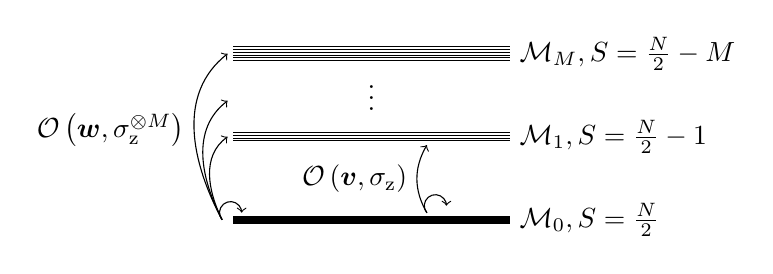
\begin{tikzpicture}
    \draw[thickest] (0,0) -- ++(10em,0);
    \foreach \hh in {0.15em,0.05em,-0.05em,-0.15em} {
      \draw (0,3em+\hh) -- ++(10em,0);
    }
    \draw[->] (7em,.25em) arc (220:0:.4em);
    \draw[->] (7em,.25em) to [bend left]
    node[left] {$\O\p{\m v,\sigma_\z}$} (7em,2.7em);
    \node () at (5em,4.7em) {$\vdots$};
    \foreach \hh in {0.25em,0.15em,0.05em,-0.05em,-0.15em,-0.25em} {
      \draw (0,6em+\hh) -- ++(10em,0);
    }
    \draw[->] (-.4em,0em) arc (220:0:.4em);
    \draw[->] (-.4em,0) to [bend left, in=130] (-.2em,3em);
    \draw[->] (-.4em,0) to [bend left, in=130] (-.2em,4.3em);
    \draw[->] (-.4em,0) to [bend left, in=130]
    node[left] {$\O\p{\m w,\sigma_\z^{\otimes M}}$} (-.2em,6em);
    \node[right] () at (10em,0) {$\M_0,S=\frac{N}{2}$};
    \node[right] () at (10em,3em) {$\M_1,S=\frac{N}{2}-1$};
    \node[right] () at (10em,6em) {$\M_M,S=\frac{N}{2}-M$};
  \end{tikzpicture}
  \caption{Schematic of relationships between $r$-magnon manifolds
    $\M_r$ with total spin $S=N/2-r$ in an SU(2) spin system.
    Single-body operators $\O\p{\m v,\sigma_\z}$ generally couple the
    ground-state manifold $\M_0$ to the single-magnon manifold $\M_1$
    as well as $\M_0$ itself, while $M$-body operators
    $\O\p{\m w,\sigma_\z^{\otimes M}}$ couple $\M_0$ to all $r$-magnon
    manifolds $\M_r$ with $r\le M$.}
  \label{fig:manifold_sketch}
\end{figure}

\red{[note: this section is not yet finished]}

\newpage

\red{[note: the remainder of this section is old, and will be replaced
  entirely]}

By construction, the $M$-body operator $X_{\m w}$ generally couples PS
states in $\M_0$ to asymmetric states in $\col\M_M$.  If the coupling
between $\M_0$ and its complement is weak compared to the spectral gap
$\Delta_{\t{gap}}$ of $H_0$, then we can treat the effect of
$X_{\m w}$ perturbatively and derive an effective Hamiltonian
$H_{\t{eff}}$ on $\M_0$.  This ground-state perturbation theory
formally breaks down when the operator norm
$\norm{X_{\m w}}\ge\Delta_{\t{gap}}/2$, in which case the operator
$X_{\m w}$ first couples $\M_0$ to $\col\M_M$, then $\col\M_M$ to
$\col\M_{2M}$, and so on.  Even if
$\norm{X_{\m w}}>\Delta_{\t{gap}}/2$, however, the energetic penalty
incurred by $H_0$ from breaking the permutational symmetry of an
initial state $\ket\psi\in\M_0$ suppresses the leakage of population
into manifolds $\M_r$ of increasing $r$.  One might therefore capture
the dynamics of an initial PS state $\ket\psi\in\M_0$ by projecting
$X_{\m w}$ onto $\col\M_{r_{\t{max}}}$ for some $r_{\t{max}}\ge M$,
resulting in a theory that resembles first-order perturbation theory
on $\col\M_{r_{\t{max}}}$.  In the perturbative regime
$\norm{X_{\m w}}<\Delta_{\t{gap}}/2$, such a theory captures all
virtual processes through order $2\floor{r_{\t{max}}/M}+1$ in a formal
perturbation theory on $\M_0$.  In the non-perturbative regime
$\norm{X_{\m w}}\ge\Delta_{\t{gap}}/2$, the error incurred by
truncating the Hilbert space of a spin system past
$\col\M_{r_{\t{max}}}$ is not clear a priori.  Nonetheless,
simulations restricted to $\col\M_{r_{\t{max}}}$ can be benchmarked by
examining the maximum populations within all $\M_r$ for
$r\le r_{\t{max}}$ throughout simulation.  As long as
\begin{enumerate*}
\item these populations fall off with increasing $r$,
\item and the maximal population within large-$r$ manifolds $\M_r$ is
  small,
\end{enumerate*}
one should expect such simulations to faithfully capture (at least
qualitatively) the dynamical behavior of the spin system under
consideration.

In order to project an operator $X_{\m w}$ onto
$\col\M_{r_{\t{max}}}$, we first need to construct a basis for
$\col\M_{r_{\t{max}}}$, and then compute all matrix elements of
$X_{\m w}$ in this basis.  Our strategy will be to first identify a
basis for $\M_0$, and then find, for each $r=1,\cdots,r_{\t{max}}$, a
suitable set of $r$-body operators $\set{O}$ and dimension-$r$ tensors
$\set{\m u}$ for which the states
$\ket{O,\m u,m}\propto O_{\m u}\ket{m}$ form an orthonormal basis for
$\M_r$.  Matrix elements of $X_{\m w}$ with respect to this basis for
$\col\M_{r_{\t{max}}}$ then take the form
\begin{align}
  \bk{O,\m u,\ell|X_{\m w}|Q,\m v,m}
  = \f{\bk{\ell|O_{\m u}^\dag X_{\m w} Q_{\m v}|m}}
  {\sqrt{\bk{\ell|O_{\m u}^\dag O_{\m u}|\ell}
      \bk{m|Q_{\m v}^\dag Q_{\m v}|m}}}.
  \label{eq:matrix_element}
\end{align}
In order to compute these matrix elements, we simplify products of the
form $\P_0 O_{\m u}^\dag X_{\m w} Q_{\m v} \P_0$ and
$\P_0 O_{\m u}^\dag O_{\m u} \P_0$, with $\P_0$ a projector onto
$\M_0$, in Appendix \ref{sec:operator_product}.

Denoting all assignments of $N$ (identical) spins to $n$ (distinct)
states by $\A_n\p{N}$, a suitable basis for $\M_0$ is the set of PS
states $\set{\ket{m}:m\in\A_n\p{N}}$, where $m=\p{m_1,m_2,\cdots,m_n}$
specifies the occupation number $m_\mu$ of each single-spin state
$\mu$.  For consistency with the expression of matrix elements in
\eqref{eq:matrix_element}, for each $\ket{m}\in\M_0$ we define
$\ket{\1,1,m}\equiv\ket{m}$, with $\1$ the identity operator, and we
define $\1_1\equiv\1$.  We now need to determine the set of $r$-body
operators $\set{O}$ and dimension-$r$ tensors $\set{\m u}$ that define
our basis for each $\M_r$.  As an initial guess for $\set{\m u}$, we
can choose the set $\set{\m u_\Delta}_{\m h,r}$ of dimension-$r$
tensors $\m u_\Delta$ that generate eigenstates of $H_0$.  The set of
$r$-body operators to choose is less obvious, but can be determined by
an exhaustive search over all $r$-body operators relevant to a
particular scenario.  Specifically, the purpose of projecting
operators onto $\col\M_{r_{\t{max}}}$ is to simulate the dynamics
induced by some operator $\hat\O$ of the form in \eqref{eq:pert},
constructed from a set $\O=\set{\p{X,\m w}}$ containing multi-spin
operators $X$.  In order to find a basis for the {\it relevant} states
in $\M_r$, one can simply consider the set $\set{O}_{\O,r}$ all
$r$-spin operators that can be constructed from products of the
multi-spin operators $X$ in $\O$.

In general, the states $\ket{O,\m u_\Delta,m}$ for all
$\p{O,\m u_\Delta,m}\in\set{O}_{\O,r}\times\set{\m u_\Delta}_{\m h,r}
\times\A_n\p{N}$ will form an overcomplete basis for the relevant
states in $\col\M_r$.  Our last step is therefore to reduce this set
of states to a minimal basis $\B_r$ for $\M_r$.  To this end, we
construct each of $\B_1,\B_2,\cdots,\B_{r_{\t{max}}}$ in sequence,
such that when constructing $\B_r$ we already have a minimal basis
$\col\B_{r-1}\equiv\bigcup_{s<r}\B_s$ for $\col\M_{r-1}$.  To
construct $\B_r$, we then consider each
$\p{O,\m u_\Delta,m}\in\set{O}_{\O,r}\times\set{\m u_\Delta}_{\m h,r}
\times\A_n\p{N}$ one at a time.  If $\ket{O,\m u_\Delta,m}$ is
orthogonal to all states in $\col\B_{r-1}$, as well as all other
states we have added to $\B_r$ thus far, then we include it in $\B_r$.
Otherwise, we discard $\ket{O,\m u_\Delta,m}$.  There are two
considerations to keep in mind for this construction: first, one
should always throw out null states $\ket{O,\m u_\Delta,m}=0$, which
can be identified by a vanishing self-overlap,
$\bk{O,\m u_\Delta,m|O,\m u_\Delta,m}=0$.  Second, computing overlaps
to check for orthogonality can be computationally intensive.  When
considering a candidate state $\ket{O,\m u_\Delta,m}$ to add to
$\B_r$, one can therefore restrict orthogonality checks to other
states $\ket{Q,\m v_\epsilon,\ell}$ with $\epsilon=\Delta$; if the
excitation energies $\epsilon\ne\Delta$, then these states are
guaranteed to be orthogonal.  Any two states with different occupation
numbers of single-spin states $\mu\in\ZZ_n$ are similarly guaranteed
to be orthogonal.

\red{[look at \cite{rai1988correlated} for classifying asymmetric
  states]}

%%%%%%%%%%%%%%%%%%%%%%%%%%%%%%%%%%%%%%%%%%%%%%%%%%%%%%%%%%%%%%%%%%%%%%
\section{Conclusions}
\label{sec:conclusions}


\red{[TODO: write section]}



\newpage
\appendix

%%%%%%%%%%%%%%%%%%%%%%%%%%%%%%%%%%%%%%%%%%%%%%%%%%%%%%%%%%%%%%%%%%%%%%
\section{Existence of a spectral gap with long-range power-law
  interactions}
\label{sec:spectral_gap}

\red{[todo: make this a subsection of Appendix
  \ref{sec:single_body_eigenstates}]}

Here we show that in $D$ spatial dimensions, power-law
SU($n$)-symmetric interactions of the form in \eqref{eq:H_0} with
$h_{ij}=-1/\abs{i-j}^\alpha$ yield a non-vanishing spectral gap when
$\alpha\le D$.  For definiteness, we will consider a periodic
hypercubic lattice of $N=L^D$ spins.  The spectral gap of the
interaction Hamiltonian is then (see Appendix
\ref{sec:single_body_eigenstates})
\begin{align}
  \Delta
  = \sum_{d\in\ZZ_L^D} h_{0,d} \sp{\cos\p{d \c k_{\t{SE}}}-1}
  = \sum_{\substack{d\in\ZZ_L^D\\\abs{d}\ge1}}
  \f{1-\cos\p{d \c k_{\t{SE}}}}{\abs{d}^\alpha},
\end{align}
where $\ZZ_L$ denotes the set of integers modulo $L$;
$k_{\t{SE}}\in\ZZ_L^D\times2\pi/L$ is a wavenumber for a single-magnon
spin-wave state; and the norm $\abs{d}$ for a vector $d$ on a periodic
lattice is implicitly understood to mean the smallest Euclidean
distance of $d$ from a fixed origin.  In order to yield the smallest
excitation energy $\Delta$, the wavenumber $k_{\t{SE}}$ should
maximize the contribution of the cosine term above, which is achieved
by a wavenumber that minimizes the oscillations of this term when
integrated over the entire lattice.  A suitable candidate for a
minimal wavenumber is $k_{\t{SE}}=\p{2\pi/L,0,0,\cdots}$, which
corresponds to an excitation energy
\begin{align}
  \Delta = \sum_{\substack{d\in\ZZ_L^D\\\abs{d}\ge1}}
  \f{1-\cos\p{d_12\pi/L}}{\abs{d}^\alpha}.
\end{align}
Defining $\epsilon\equiv2/L$ and a rescaled domain symmetrized about
$0$, $\SS_\epsilon\simeq\ZZ_L/\epsilon$ with
$\SS_\epsilon\subset\sp{-1,1}$, we substitute $x\simeq\epsilon d$ to
get
\begin{align}
  \Delta
  = \sum_{\substack{x\in\SS_\epsilon^D\\\abs{x}\ge\epsilon}}
  \f{1-\cos\p{\pi x_1}}{\abs{x/\epsilon}^\alpha}
  = \epsilon^{\alpha-D} \sum_{\substack{x\in\SS_L^D\\\abs{x}\ge\epsilon}}
  \epsilon^D \f{1-\cos\p{\pi x_1}}{\abs{x}^\alpha}.
\end{align}
As $\epsilon\to0$ the discrete sum over $x$ is well approximated by an
integral that avoids an infinitesimal region about the origin, i.e.
\begin{align}
  \Delta = \epsilon^{\alpha-D} \I_D\p{\epsilon},
  &&
  \I_D\p{\epsilon}
  \equiv \int_{\TT_1^D\setminus\TT_\epsilon^D} \d^Dx\,
  \f{1-\cos\p{\pi x_1}}{\abs{x}^\alpha},
\end{align}
where the integral $\I_D\p{\epsilon}$ is defined using the symmetric
interval $\TT_a\equiv\p{-a/2,a/2}$.  The integrand of
$\I_D\p{\epsilon}$ is strictly positive and well-behaved on the
entirety of its domain except for the origin, where depending on the
value of $\alpha$ the integrand may vanish or diverge as
$\abs{x}\to0$.  Together, these facts mean that
\begin{align}
  \I_D\p{\epsilon} \stackrel{\epsilon\to0}{\sim} \epsilon^{-\gamma},
  &&
  \Delta \stackrel{\epsilon\to0}{\sim} \epsilon^{\alpha-D-\gamma},
\end{align}
for some $\gamma\ge0$, which implies that gap $\Delta$ is
non-vanishing when $\alpha\le D\le D+\gamma$.

For the sake of completion, we add that in fact the gap $\Delta$
always vanishes in the thermodynamic limit when $\alpha>D$.  To see
this behavior, we note that the asymptotic dependence of the integral
$\I_D\p{\epsilon}$ on $\epsilon$ is determined by the behavior of its
integrand when $\abs{x}\sim\epsilon$, in which case
$1-\cos\p{\pi x_1}\sim x_1^2$, so
\begin{align}
  \I_D\p{\epsilon}
  \sim \int_{\TT_1^D\setminus\TT_\epsilon^D} \d^Dx\,
  \f{x_1^2}{\abs{x}^\alpha}.
\end{align}
We can then use the fact that $x_1^2\le\abs{x}^2$ and change to
spherical coordinates to find that
\begin{align}
  \I_D\p{\epsilon} \lesssim
  \int_{\TT_1^D\setminus\TT_\epsilon^D} \d^Dx\,
  \f{\abs{x}^2}{\abs{x}^\alpha}
  \sim \int_\epsilon^1 \d x\, x^{D+1-\alpha}
  \sim
  \begin{cases}
    \epsilon^0 & \alpha < D+2 \\
    \log\p{1/\epsilon} & \alpha = D+2 \\
    \epsilon^{D+2-\alpha} & \alpha > D+2
  \end{cases}.
\end{align}
It follows that the spectral gap
\begin{align}
  \Delta \stackrel{\epsilon\to0}{\lesssim}
  \begin{cases}
    \epsilon^{\alpha-D} & \alpha < D+2 \\
    \epsilon^2 \log\p{1/\epsilon} & \alpha = D + 2 \\
    \epsilon^2 & \alpha > D+2
  \end{cases},
\end{align}
which vanishes as $\epsilon\to0$ for all $\alpha>D$.

%%%%%%%%%%%%%%%%%%%%%%%%%%%%%%%%%%%%%%%%%%%%%%%%%%%%%%%%%%%%%%%%%%%%%%
\section{Generating excitation energy eigenstates}
\label{sec:eigenstates}

Both perturbation theory and beyond-perturbative simulations of the
dynamics induced by an operator $\O\p{\m w,X}$ require us to decompose
$\O\p{\m w,X}$ into a sum of terms that generate eigenstates of the
SU($n$)-symmetric interaction Hamiltonian $H_0$ in \eqref{eq:H_0} when
acting on permutationally symmetric (PS) states $\ket\psi\in\M_0$.  To
perform this decomposition, in this section we simplify products of
the form $H_0\O\p{\m w,X}\ket\psi$ with $\ket\psi\in\M_0$.  For
reference, the $M$-body operator $\O\p{\m w,X}$ is defined by
\begin{align}
  \O\p{\m w,X} \equiv \sum_{k\in\D_N\p{M}} w_k X_k,
\end{align}
where $\m w$ is a dimension-$M$ (i.e.~$M$-index) tensor of scalar
coefficients $w_k\equiv w_{k_1k_2\cdots k_M}$; $X$ is an $M$-spin
operator; $k\equiv\p{k_1,k_2,\cdots,k_M}$ is a list of the individual
spins $k_i\in\ZZ_N$ that the operator $X_k\equiv X_{k_1k_2\cdots k_M}$
acts on; and
\begin{align}
  \D_N\p{M} \equiv
  \set{ k \in \ZZ_N^M: \t{all entries $k_i$ of $k$ are distinct} },
\end{align}
is the strictly ``off-diagonal'' part of $\ZZ_N^M$.

%%%%%%%%%%%%%%%%%%%%%%%%%%%%%%%%%%%%%%%%%%%%%%%%%%
\subsection{Single-body excitations}
\label{sec:single_body_eigenstates}

To build familiarity with the problem at hand, we first consider the
simple case of a single-body ($M=1$) case and simplify
\begin{align}
  H_0 \O\p{\m w,X} \ket\psi
  = \f12 \sum_{i\ne j} \sum_k h_{ij} w_k \Pi_{ij} X_k \ket\psi.
  \label{eq:single_body_diagnosis_start}
\end{align}
The sum in \eqref{eq:single_body_diagnosis_start} has terms with
$k\in\set{i,j}$, and terms with $k\notin\set{i,j}$.  In the case of
$k\notin\set{i,j}$, the permutation operator $\Pi_{ij}$ commutes with
$X_k$ and annihilates on $\ket\psi$, and we can replace the sum
\begin{align}
  \sum_{k\notin\set{i,j}} \to \sum_k - \sum_{k\in\set{i,j}},
\end{align}
allowing us to simplify
\begin{align}
  \f12 \sum_{i\ne j} \sum_{k\notin\set{i,j}}
  h_{ij} w_k \Pi_{ij} X_k \ket\psi
  = E_0 \O\p{\m w,X} \ket\psi
  - \f12 \sum_{i\ne j} \sum_{k\in\set{i,j}} h_{ij} w_k X_k \ket\psi,
\end{align}
where $E_0=\frac12\sum_{i\ne j}h_{ij}$ is the interaction energy of PS
states $\ket\psi\in\M_0$.  Making the replacement
\begin{align}
  \sum_{i\ne j} \sum_{k\in\set{i,j}}
  \to \sum_k \sum_{\substack{i\ne j\\\set{i,j}\ni k}},
\end{align}
we can simplify
\begin{align}
  \f12 \sum_{\substack{i\ne j\\\set{i,j}\ni k}} h_{ij}
  = \f12 \sum_i h_{ik} + \f12 \sum_j h_{kj}
  = h_k,
  &&
  h_k \equiv \sum_i h_{ik},
\end{align}
which implies that the terms in \eqref{eq:single_body_diagnosis_start}
with $k\notin\set{i,j}$ are
\begin{align}
  \f12 \sum_{i\ne j} \sum_{k\notin\set{i,j}}
  h_{ij} w_k \Pi_{ij} X_k \ket\psi
  = E_0 \O\p{\m w,X} \ket\psi - \sum_k h_k w_k X_k \ket\psi.
\end{align}
The terms in \eqref{eq:single_body_diagnosis_start} with
$k\in\set{i,j}$, meanwhile, are
\begin{align}
  \f12 \sum_{\substack{i\ne j\\k\in\set{i,j}}}
  h_{ij} w_k \Pi_{ij} X_k \ket\psi
  = \sum_{j,k} h_{kj} w_k X_j \ket\psi.
\end{align}
so in total
\begin{align}
  H_0 \O\p{\m w,X} \ket\psi
  = E_0 \O\p{\m w,X} \ket\psi
  + \sum_k \sp{\sum_j h_{kj} w_j - h_k w_k} X_k \ket\psi.
  \label{eq:single_body_diagnosis_end}
\end{align}
The action of the single-body perturbation $\O\p{\m w,X}$ on a
permutationally symmetric state therefore generates an eigenstate of
$H_0$ with energy $E_0+\Delta$ if the vector $\m w=\sum_k w_k \ket{k}$
satisfies the eigenvalue equation
\begin{align}
  \p{\m h - \oper{diag}\v h} \c \m w = \Delta \m w,
  \label{eq:single_body_eig}
\end{align}
where $\m h\equiv\sum_{i,j} h_{ij} \op{i}{j}$ is a matrix of all
couplings $h_{ij}$; the vector
$\v h \equiv \sum_{i,j} h_{ij} \ket{i} = \sum_i h_i \ket{i}$ is the
sum of all columns of $\m h$; and $\oper{diag}\v h$ is a matrix with $\v h$
on the diagonal and zeroes everywhere else.  When the interaction
Hamiltonian $H_0$ is translationally invariant, the single-body
eigenvalue problem in \eqref{eq:single_body_eig} is solvable
analytically.  In this case, the couplings $h_{ij}$ depend only on the
separation $\abs{i-j}$, so eigenvectors of $\m h$ are plane waves of
the form
\begin{align}
  \m w_k \equiv \sum_{d\in\ZZ_L^D} e^{\i d\c k} \ket{d},
\end{align}
where on a $D$-dimensional periodic lattice of $N=L^D$ spins, lattice
sites are indexed by vectors $d\in\ZZ_L^D$, and wavenumbers take on
values $k\in\ZZ_L^D\times2\pi/L$.  The corresponding eigenvalues of
$\m h$ can be determined by expanding
\begin{align}
  \m h \c \m w_k
  = \sum_{c,d\in\ZZ_L^D} h_{cd} e^{\i d\c k} \ket{c}
  = \sum_{c,d\in\ZZ_L^D} h_{c,c+d} e^{\i\p{c+d}\c k} \ket{c}
  = \sum_{d\in\ZZ_L^D} h_{0,d} \cos\p{d\c k} \m w_k,
\end{align}
where the imaginary contributions vanish in the sum over $d$ because
$h_{0,d}=h_{0,-d}$.  The remainder of \eqref{eq:single_body_eig} that
we need to sort out is $\oper{diag}\v h$, where all
$h_i = \sum_{i,j}h_{ij} = \sum_d h_{0,d}$ are equal, which implies
that $\oper{diag}\v h = \sum_d h_{0,d}$ is a scalar.  We thus find that
\begin{align}
  \p{\m h - \oper{diag}\v h} \c \m w_k = \Delta_k \m w_k,
  &&
  \Delta_k \equiv \sum_{d\in\ZZ_L^D} h_{0,d} \sp{\cos\p{d\c k}-1}.
\end{align}

%%%%%%%%%%%%%%%%%%%%%%%%%%%%%%%%%%%%%%%%%%%%%%%%%%
\subsection{Multi-body excitations}

We now consider the full $M$-body case
\begin{align}
  H_0 \O\p{\m w,X} \ket\psi
  = \sum_{\substack{k\in\D_N\p{M}\\\set{i,j}\in\C_N\p{2}}}
  h_{ij} w_k \Pi_{ij} X_k \ket\psi,
  \label{eq:diagnosis_start}
\end{align}
where for convenience we define
\begin{align}
  \C_N\p{q} \equiv \set{ s \subset \ZZ_N : \abs{s} = q }
  \label{eq:choices}
\end{align}
as the set of all subsets (``choices'') of $q$ elements from $\ZZ_N$.
The sum in \eqref{eq:diagnosis_start} has terms with $i,j\notin k$,
terms with $i,j\in k$, and terms with only one of $i$ or $j\in k$.
The permutation operator $\Pi_{ij}$ acts trivially on $X_k\ket\psi$
when $i,j\notin k$, and we can replace the sum
\begin{align}
  \sum_{\substack{\set{i,j}\in\C_N\p{2}\\i,j\notin k}}
  \to \sum_{\set{i,j}\in\C_N\p{2}}
  - \sum_{\substack{\set{i,j}\in\C_N\p{2}\\i\in k~\t{or}~j\in k}},
\end{align}
allowing us to simplify
\begin{align}
  \sum_{k\in\D_N\p{M}} \sum_{\substack{\set{i,j}\in\C_N\p{2}\\i,j\notin k}}
  h_{ij} w_k \Pi_{ij} X_k \ket\psi
  = E_0 \O\p{\m w,X} \ket\psi
  - \sum_{k\in\D_N\p{M}} h^{\t{D}}_k w_k X_k \ket\psi,
\end{align}
where $E_0 = \sum_{\set{i,j}\in\C_N\p{2}} h_{ij}$ is the interaction
energy of PS states $\ket\psi\in\M_0$, and
\begin{align}
  h^{\t{D}}_k \equiv
  \sum_{\substack{\set{i,j}\in\C_N\p{2}\\i\in k~\t{or}~j\in k}} h_{ij}
  = \sum_{i\in k} h_i - \sum_{\set{a,b}\in\C_M\p{2}} h_{k_ak_b},
  &&
  h_i \equiv \sum_j h_{ij},
  \label{eq:multi_body_op_diag_element}
\end{align}
with $k_a,k_b\in k\equiv\p{k_1,k_2,\cdots,k_M}$.  Defining a linear
operator $\hat{\m h}_{\t{D}}$ on the space of dimension-$M$ tensors,
whose action on $\m w$ is a new dimension-$M$ tensor with entries
\begin{align}
  \p{\hat{\m h}_{\t{D}}\c\m w}_k \equiv h^{\t{D}}_k w_k,
  \label{eq:multi_body_op_diag}
\end{align}
we can write the terms in \eqref{eq:diagnosis_start} with
$i,j\notin k$ as
\begin{align}
  \sum_{k\in\D_N\p{M}} \sum_{\substack{\set{i,j}\in\C_N\p{2}\\i,j\notin k}}
  h_{ij} w_k \Pi_{ij} X_k \ket\psi
  = E_0 \O\p{\m w,X} \ket\psi
  - \sum_{k\in\D_N\p{M}} \p{\hat{\m h}_{\t{D}}\c\m w}_k X_k \ket\psi.
\end{align}
The terms in \eqref{eq:diagnosis_start} with $i,j\in k$ are
\begin{align}
  \sum_{k\in\D_N\p{M}} \sum_{\substack{\set{i,j}\in\C_N\p{2}\\i,j\in k}}
  h_{ij} w_k \Pi_{ij} X_k \ket\psi
  = \sum_{k\in\D_N\p{M}} \sum_{\substack{\set{a,b}\in\C_M\p{2}}}
  h_{k_ak_b} w_{k_{a\lra b}} X_k \ket\psi,
\end{align}
where $k_{a\lra b}$ denotes a list that is equal to
$k=\p{k_1,k_2,\cdots,k_M}$ but with $k_a$ and $k_b$ swapped, and we
have relabeled $k_a$ and $k_b$ to change $w_k X_{k_{a\lra b}}$ to
$w_{k_{a\lra b}} X_k$.  To write down these terms succinctly, we
define a linear operator $\hat{\m h}_{\t{P}}$ on the space of
dimension-$M$ tensors, whose action on $\m w$ is a new dimension-$M$
tensor with entries
\begin{align}
  \p{\hat{\m h}_{\t{P}} \c \m w}_k
  \equiv \sum_{\substack{\set{a,b}\in\C_M\p{2}}}
  h_{k_ak_b} w_{k_{a\lra b}},
  \label{eq:multi_body_op_perm}
\end{align}
such that
\begin{align}
  \sum_{k\in\D_N\p{M}} \sum_{\substack{\set{i,j}\in\C_N\p{2}\\i,j\in k}}
  h_{ij} w_k \Pi_{ij} X_k \ket\psi
  = \sum_{k\in\D_N\p{M}} \p{\hat{\m h}_{\t{P}} \c \m w}_k X_k \ket\psi.
\end{align}
Finally, the terms in \eqref{eq:diagnosis_start} with only one of
$i\in k$ or $j\in k$ are
\begin{align}
  \sum_{k\in\D_N\p{M}} \sum_{i\notin k} \sum_{j\in k}
  h_{ij} w_k \Pi_{ij} X_k \ket\psi
  = \sum_{k\in\D_N\p{M}} \sum_{i\notin k}
  \sum_{a\in\ZZ_M} h_{ik_a} w_{k_{a:i}} X_k \ket\psi,
\end{align}
where $k_{a:i}$ denotes a list that is equal to $k$ but with $k_a$
replaced by $i$, and we have relabeled $k_a$ and $i$ to change
$w_k X_{k_{a:i}}$ to $w_{k_{a:i}} X_k$.  For each fixed $a$, the sum
over $i$ above is essentially a contraction of the matrix $\m h$ with
the $a$-th index of the tensor $\m w$.  Defining a linear operator
$\hat{\m h}_a$ on the space of dimension-$M$ tensors, whose action on
$\m w$ is a new dimension-$M$ tensor with entries
\begin{align}
  \p{\hat{\m h}_a\c\m w}_k
  \equiv \sum_{i\notin k} h_{ik_a} w_{k_{a:i}}
  = \sum_{i\notin k}
  h_{ik_a} w_{k_1 k_2 \cdots k_{a-1} i k_{a+1} \cdots k_M},
  \label{eq:multi_body_op_contract}
\end{align}
we can expand
\begin{align}
  \sum_{k\in\D_N\p{M}} \sum_{i\notin k} \sum_{j\in k}
  h_{ij} w_k \Pi_{ij} X_k \ket\psi
  = \sum_{k\in\D_N\p{M}} \sum_{a\in\ZZ_M}
  \p{\hat{\m h}_a\c\m w}_k X_k \ket\psi.
\end{align}
Altogether, defining the combined operator
\begin{align}
  \hat{\m h}
  \equiv \sum_{a\in\ZZ_M} \m h_a + \m h_{\t{P}} - \m h_{\t{D}},
\end{align}
we find that
\begin{align}
  H_0 \O\p{\m w,X} \ket\psi
  = E_0 \O\p{\m w,X} \ket\psi +
  \O\p{\hat{\m h}\c\m w, X} \ket\psi
  = \sum_\Delta \p{E_0+\Delta} \O\p{\m w_\Delta, X} \ket\psi,
\end{align}
where $\m w_\Delta$ is the projection of $\m w$ onto the eigenspace of
$\hat{\m h}$ with eigenvalue $\Delta$, i.e.
\begin{align}
  \hat{\m h} \c \m w_\Delta = \Delta \m w_\Delta,
  \label{eq:multi_body_problem}
\end{align}
with
\begin{align}
  \hat{\m h} \equiv \sum_{k\in\D_N\p{M}} \ket{k}
  \sp{\sum_{a\in\ZZ_M} \sum_{\substack{i\in\ZZ_N\\i\notin k}}
    h_{ik_a} \bra{k_{a:i}}
    + \sum_{\set{a,b}\in\C_M\p{2}} h_{k_ak_b} \bra{k_{a\lra b}}
    - h^{\t{D}}_k \bra{k}}.
  \label{eq:multi_body_mat}
\end{align}
For reference, here $k_{a:i}$ is equal to
$k\equiv\p{k_1,k_2,\cdots,k_M}$ but with $k_a$ replaced by $i$;
$\C_M\p{2}$ is defined in \eqref{eq:choices}; $k_{a\lra b}$ is equal
to $k$ but with $k_a$ and $k_b$ swapped; and $h^{\t{D}}_k$ is defined
in \eqref{eq:multi_body_op_diag_element}.

If the coefficient tensor $\m w$ is permutationally symmetric, meaning
that $\m w$ is invariant under arbitrary permutations of its tensor
factors, then this symmetry is preserved by $\hat{\m h}$.  In this
case, we can replace sums over $k\in\D_N\p{M}$ in
\eqref{eq:multi_body_problem} and \eqref{eq:multi_body_mat} by sums
over $k\in\C_N\p{M}$, and replace vectors
$\ket{k_1,k_2,\cdots,k_M}\to\ket{\set{k_1,k_2,\cdots,k_M}}$, such that
e.g.~$\ket{k_{a\lra b}}=\ket{k}$.  These replacements reduce the size
of $\hat{\m h}$ from $\abs{\D_N\p{M}}\times\abs{\D_N\p{M}}$ to
$\abs{\C_N\p{M}}\times\abs{\C_N\p{M}}$, where
$\abs{\D_N\p{M}}=\prod_{j=0}^{M-1}\p{N-j}=M!\times{N\choose M}$ and
$\abs{\C_N\p{M}}={N\choose M}$.  We discuss further reduction of the
eigenvalue problem in \eqref{eq:multi_body_problem} by use of
additional symmetries in Section \ref{sec:symmetries}.

Some special cases of practical interest: if $M=1$, then
$h^{\t{D}}_k=h_k$, so
\begin{align}
  \hat{\m h} \stackrel{M=1}{=} \sum_{k\in\ZZ_N} \ket{k}
  \sp{\sum_{i\in\ZZ_N} h_{ik} \bra{i} - h_k \bra{k}}
  = \m h - \oper{diag}\v h,
\end{align}
which is precisely what we found in \eqref{eq:single_body_eig}.  If
$M=2$, then $h_{k\ell}^{\t{D}}=h_k+h_\ell-h_{k\ell}$, so
\begin{align}
  \hat{\m h} \stackrel{M=2}{=}
  \sum_{\p{k,\ell}\in\D_N\p{2}} \ket{k\ell}
  \sp{\sum_{\substack{i\in\ZZ_N\\i\notin\set{k,\ell}}}
    \p{ h_{ik} \bra{i\ell} + h_{i\ell} \bra{ki} }
    + h_{k\ell} \bra{\ell k}
    - \p{h_k + h_\ell - h_{k\ell}} \bra{k\ell}}.
\end{align}

%%%%%%%%%%%%%%%%%%%%%%%%%%%%%%%%%%%%%%%%%%%%%%%%%%
\subsection{Exploiting spatial symmetries}
\label{sec:symmetries}

Solving the eigenvalue problem in \eqref{eq:multi_body_problem} to
find $M$-body operators $\O\p{\m w_\Delta,X}$ that generate states of
definite interaction energy nominally requires diagonalizing the
matrix $\hat{\m h}$ with dimensions $\sim N^M\times N^M$.  Spatial
symmetries of the interaction Hamiltonian $H_0$, however, generally
endow $\hat{\m h}$ with a block-diagonal structure that can be used to
reduce the complexity of this eigenvalue problem.  Translational
invariance, for example, can reduce this problem to that of
diagonalizing a matrix with dimensions $\sim N^{M-1}\times N^{M-1}$,
and isotropy can further reduce the problem size by factors that
depend on the lattice geometry.  The complexity of diagonalizing a
matrix with dimensions $d\times d$ is $O\p{d^3}$, so even a reduction
of $d$ by a factor of 2 yields practically significant gains (a factor
of $2^3=8$) in the runtime of diagonalization.  Here, we provide a
general prescription for exploiting the spatial symmetries of $H_0$ to
simplify the eigenvalue problem in \eqref{eq:multi_body_problem}.

Our task is essentially to express the multi-body eigenvalue problem
in \eqref{eq:multi_body_problem} in a basis that respects the spatial
symmetries of $H_0$.  These symmetries essentially break the set
$\D_N\p{M}$ into equivalence classes $\S_M$\footnote{For brevity, we
  will suppress the explicit dependence of $\S_M$ on $N$, as well as
  other factors such as lattice geometry.}, where elements $s\in\S_M$
are subsets $s\subset\D_N\p{M}$ that are invariant under the
appropriate symmetry group action.  In the case of $M=2$ in a
translationally invariant and isotropic system, for example, each
equivalence class $s\in\S_2$ would consist of all pairs
$\p{i,j}\in\D_N\p{2}$ that are a fixed distance $\abs{i-j}=d_s$ apart,
i.e.~$s=\set{\p{i,j}\in\D_N\p{2}:\abs{i-j}=d_s}$.  If the tensor
$\m w$ is invariant under arbitrary permutations of its tensor
factors, this symmetry is preserved by $\hat{\m h}$, and we can place
all $k\in\D_N\p{M}$ that are equal up to permutation into the same
equivalence class.

For simplicity, we first assume that the $M$-body operator
$\O\p{\m w,X}$ obeys the same spatial symmetries as $H_0$.  For any
equivalence class $s\in\S_M$, we then define a uniform superposition
$\ket{s}$ over all $k\in s$, as well as a projector $\P_\S$ onto the
space of uniform superpositions:
\begin{align}
  \ket{s} \equiv \f1{\sqrt{\abs{s}}} \sum_{k\in s} \ket{k},
  &&
  \P_{\S_M} \equiv \sum_{s\in\S_M} \op{s},
\end{align}
where $\abs{s}$ is the number of elements in $s$.  In turn, we expand
a vector of $M$-body operator coefficients
$\m w=\sum_{k\in\D_N\p{M}}w_k\ket{k}$ in this symmetrized basis:
\begin{align}
  \m w = \P_{\S_M} \m w
  = \sum_{s\in\S_M} \sum_{k\in s} w_k \ket{s} \bk{s|k}
  = \sum_{s\in\S_M} w_s \sqrt{\abs{s}} \ket{s},
\end{align}
where all $w_k$ with $k\in s$ are equal by assumption, so
$w_s\equiv\sum_{k\in s}w_k/\abs{s}=w_\ell$ for any $\ell\in s$.
Finally, we expand the projection of $\hat{\m h}$ onto the symmetric
subspace:
\begin{align}
  \P_{\S_M} \hat{\m h} \P_{\S_M}
  = \sum_{s\in\S_M} \f{\ket{s}}{\sqrt{\abs{s}}} \sp{
    \sum_{\substack{k\in s\\a\in\ZZ_M}}
    \sum_{\substack{p\in\ZZ_N\\p\notin k}}
    h_{p k_a} \f{\bra{\sp{k_{a:p}}}}{\sqrt{\abs{\sp{k_{a:p}}}}}
    + \sum_{\set{a,b}\in\C_M\p{2}} h_{k_ak_b}
    \f{\bra{\sp{k_{a\lra b}}}}{\sqrt{\abs{\sp{k_{a\lra b}}}}}
    - h^{\t{D}}_s \f{\bra{s}}{\sqrt{\abs{s}}}},
\end{align}
where $h^{\t{D}}_s\equiv h^{\t{D}}_k$ for any $k\in s$, with
$h^{\t{D}}_k$ defined in \eqref{eq:multi_body_op_diag_element}; and
$\sp{k}$ denotes the equivalence class of $k$.  The reduced multi-body
eigenvalue problem is then
\begin{align}
  \P_{\S_M} \hat{\m h} \P_{\S_M} \c \m w = \Delta \m w.
\end{align}
More generally, even if the couplings $\m w$ of $\O\p{\m w,X}$ do not
obey the spatial symmetries as $H_0$, these symmetries still endow
$\hat{\m h}$ with a block-diagonal structure that reduces the
complexity of the multi-body eigenvalue problem.  We leave this
reduction to future work.  % todo: perform reduction

%%%%%%%%%%%%%%%%%%%%%%%%%%%%%%%%%%%%%%%%%%%%%%%%%%%%%%%%%%%%%%%%%%%%%%
\section{Permutation-symmetrized products of multi-body operators}
\label{sec:operator_product}

\red{[TODO: write introductory text for this section]}

%%%%%%%%%%%%%%%%%%%%%%%%%%%%%%%%%%%%%%%%%%%%%%%%%%
\subsection{A diagrammatic expansion}

Given a system of $N$ spins, we wish to project a product of
multi-body operators onto the permutationally symmetric (PS) manifold
$\M_0$.  For $p$ multi-body operators, such a product takes the form
\begin{align}
  \Q\p{\m w,\m X}
  \equiv \prod_{\alpha\in\ZZ_p} \O\p{w_\alpha,X_\alpha}
  = \prod_{\alpha\in\ZZ_p} \sum_{k_\alpha\in\D_N\p{M_\alpha}}
  w_\alpha\p{k_\alpha} X_\alpha\p{k_\alpha},
  \label{eq:sym_prod_start}
\end{align}
where $\m w\equiv\p{w_1,w_2,\cdots,w_p}$ is a vector of
dimension-$M_\alpha$ tensors $w_\alpha$;
$\m X\equiv\p{X_1,X_2,\cdots,X_p}$ is a vector of $M_\alpha$-spin
operators $X_\alpha$;
$k_\alpha=\p{k_{\alpha,1},k_{\alpha,2},\cdots,k_{\alpha,M_\alpha}}$ is
a choice of $M_\alpha$ spins that $X_\alpha\p{k_\alpha}$ acts on;
$w_\alpha\p{k_\alpha}$ is a scalar entry of $w_\alpha$; and
$\D_N\p{M_\alpha}$ is the strictly off-diagonal part of $\ZZ_N^M$,
defined in \eqref{eq:off_diags}.  For later convenience, we extend the
definitions of $w_\alpha\p{k_\alpha}=X_\alpha\p{k_\alpha}$ to all
$k_\alpha\in\ZZ_N^M$ by defining
$w_\alpha\p{k_\alpha}=X_\alpha\p{k_\alpha}=0$ for any $k_\alpha$ with
repeated entries.

To simplify $\Q\p{\m w,\m X}$, we first collect terms to express
\eqref{eq:sym_prod_start} as a sum of products:
\begin{align}
  \Q\p{\m w,\m X} = \sum_{k\in\D_N\p{\m M}} \prod_{\alpha\in\ZZ_p}
  w_\alpha\p{k_\alpha} X_\alpha\p{k_\alpha},
  \label{eq:sym_prod_sum}
\end{align}
where $\m M\equiv\p{M_1,M_2,\cdots,M_p}$ is a vector of the dimensions
$M_\alpha$; and
$\D_N\p{\m M}\equiv\bigotimes_{M_\alpha\in\m M}\D_N\p{M_\alpha}$, such
that each $k\in\D_N\p{\m M}$ has the decomposition
$k=\p{k_1,k_2,\cdots,k_p}$ with $k_\alpha\in\D_N\p{M_\alpha}$.  We
then classify the terms in \eqref{eq:sym_prod_sum} by the numbers
$g_S$ of indices shared by all tensors $w_\alpha$ with
$\alpha\in S\subset\ZZ_p$.  For example, a term of the form
$w_1\p{a,b,c} w_2\p{b,d,e} w_3\p{b,c,d,e}$ with distinct indices
$a,b,c,d,e$ would have
\begin{align}
  g_{\set{1}} = 1,
  &&
  g_{\set{1,2,3}} = 1,
  &&
  g_{\set{1,3}} = 1,
  &&
  g_{\set{2,3}} = 2,
\end{align}
and $g_S=0$ for all other subsets $S\subset\ZZ_3$.  This index
assignment can be associated with the Venn diagram
\begin{align}
  \diagram{example_123},
  \label{eq:venn_diagram}
\end{align}
where $g_S$ is determined the number of dots at the intersection of
circles $\alpha\in S$.  We denote the set of all nonempty subsets of
$\ZZ_p$ by $\PP^*\p{\ZZ_p}$, and denote a choice of $g_S$ for all
$S\in\PP^*\p{\ZZ_p}$ by $g$.  With representations such as
\eqref{eq:venn_diagram} in mind, we will loosely refer to $g$ as
simply a ``diagram''.  We define
$\abs{g}\equiv\sum_{S\in\PP^*\p{\ZZ_p}}g_S$ to be the number of
indices considered in $g$ (or equivalently the number of dots in the
diagram $g$), and we denote the set of all diagrams for
$p=\dim\p{\m M}$ tensors with dimensions $\m M$ by $\G\p{\m M}$.  For
consistency, all diagrams $g\in\G\p{\m M}$ must associate exactly
$M_\alpha$ indices with the dimension-$M_\alpha$ tensor $w_\alpha$,
i.e.
\begin{align}
  \sum_{S\in\PP^*\p{\ZZ_p}\,:\,\alpha\in S} g_S
  = \sum_{R\in\PP^*\p{\ZZ_p\setminus\set{\alpha}}} g_{\set{\alpha}\cup R}
  = M_\alpha
\end{align}
for all $\alpha\in\ZZ_p$.  A classification of the terms in
\eqref{eq:sym_prod_start} by diagrams $g\in\G\p{\m M}$ allows us to
expand
\begin{align}
  \Q\p{\m w,\m X} \EQPS \sum_{g\in\G\p{\m M}} \Q_g\p{\m w,\m X},
  \label{eq:sym_prod_diagrams}
\end{align}
where $\EQPS$ denotes equality under a restriction to $\M_0$, and
$\Q_g\p{\m w,\m X}$ is the sum of all terms in
\eqref{eq:sym_prod_start} that are associated with the diagram $g$.

To find an explicit form of $\Q_g\p{\m w,\m X}$, we first consider all
distinct ways to assign $\abs{g}$ indices to specific tensor factors
of $\m w$ and $\m X$ in a manner consistent with $g$.  For example, if
$\m X=\p{X_1,X_2}$ with dimensions $\p{M_1,M_2}=\p{2,1}$ and
$\abs{g}=2$ with $g_{\set{1}}=g_{\set{1,2}}=1$, then
$X_1\p{a,b} X_2\p{b}$ and $X_1\p{b,a} X_2\p{b}$ are distinct
assignments of $\abs{g}$ indices to $\m X$ in a manner consistent with
$g$, provided that $a\ne b$.  After assigning $\abs{g}$ indices to
$\m w$ and $\m X$ in a manner consistent with $g$, we need to sum over
all values that these indices can take, which amounts to a sum over
all $k\in\D_N\p{\abs{g}}$.

A specific assignment of indices can be thought of as a choice, for
each of the $M_\alpha$ tensor factors of $w_\alpha$ and $X_\alpha$, of
which dot in the diagram $g$ that tensor factor is associated with
(i.e.~out of the $M_\alpha$ dots within circle $\alpha$).  There are
nominally $M_\alpha!$ such choices for a given $\alpha$, and therefore
$\prod_{\alpha\in\ZZ_p}M_\alpha!$ choices total.  The only catch is
that these choices treat all dots in $g$ as distinct, whereas the
$g_S$ dots within region $S$ of $g$ are actually indistinguishable.
The assignment $X_1\p{a,b,c} X_2\p{a,b}$, for example, is the same as
$X_1\p{b,a,c} X_2\p{b,a}$, because $a$ and $b$ are dummy indices.
Treating $g_S$ dummy indices as as distinguishable results in
over-counting distinct index assignments by a factor of $g_S!$.
Denoting the set of all distinct index assignments according to $g$ by
$\L\p{g}$, the number of such assignments is therefore
\begin{align}
  \abs{\L\p{g}} = \sp{\prod_{\alpha\in\ZZ_p}M_\alpha!}
  \times \sp{\prod_{S\in\PP^*\p{\ZZ_p}} g_S!}^{-1}.
  \label{eq:symmetry}
\end{align}
Altogether, we have
\begin{align}
  \Q_g\p{\m w,\m X} \equiv
  \sum_{\ell\in\L\p{g}} \sum_{k\in\D_N\p{\abs{g}}}
  \m w\p{k,\ell} \m X\p{k,\ell},
\end{align}
where $\m w\p{k,\ell}$ and $\m X\p{k,\ell}$ denote the scalar and
operator acquired by assigning the indices
$k=\p{k_1,k_2,\cdots,k_{\abs{g}}}$ to $\m w$ and $\m X$ according to
$\ell$.  Upon projection to the PS manifold $\M_0$, this operator
becomes
\begin{align}
  \Q_g\p{\m w,\m X} \equiv
  \sum_{\ell\in\L\p{g}} \col{\m w}\p{\ell} \mean{\m X}\p{\ell},
  \label{eq:sum_assignments}
\end{align}
where
\begin{align}
  \col{\m w}\p{\ell} \equiv \sum_{k\in\D_N\p{\abs{g}}} \m w\p{k,\ell},
  &&
  \mean{\m X}\p{\ell}
  \equiv \f1{\abs{\D_N\p{\abs{g}}}}
  \sum_{k\in\D_N\p{\abs{g}}} \m X\p{k,\ell},
\end{align}
and permutational symmetry implies that the averaging for
$\mean{\m X}\p{\ell}$ is not actually necessary:
\begin{align}
  \mean{\m X}\p{\ell}
  \EQPS \m X\p{k,\ell} ~\t{for any}~ k\in\D_N\p{\abs{g}}.
\end{align}
If, furthermore, all tensors $w_\alpha$ in $\m w$ (or all operators
$X_\alpha$ in $\m X$) are permutationally symmetric, meaning that they
are invariant under arbitrary permutations of their tensor factors,
then
\begin{align}
  \Q_g\p{\m w,\m X}
  \stackrel{\t{sym}}{=}_{\t{PS}} \col{\m w}\p{g} \mean{\m X}\p{g},
  \label{eq:sum_diagrams}
\end{align}
where $\stackrel{\t{sym}}{=}_{\t{PS}}$ denotes equality up to
\begin{enumerate*}
\item permutational symmetry of all $\m w$ or $\m X$, and
\item restriction to the PS manifold $\M_0$; and
\end{enumerate*}
\begin{align}
  \col{\m w}\p{g} \equiv \sum_{\ell\in\L\p{g}} \col{\m w}\p{\ell},
  &&
  \mean{\m X}\p{g} \equiv \f1{\abs{\L\p{g}}}
  \sum_{\ell\in\L\p{g}} \mean{\m X}\p{\ell}.
\end{align}
In summary, the product of operators $\Q\p{\m w,\m X}$ in
\eqref{eq:sym_prod_start} admits the diagrammatic expansion in
\eqref{eq:sym_prod_diagrams}, as a sum of $\Q_g\p{\m w,\m X}$ over all
diagrams $g\in\G\p{\m M}$.  Each term $\Q_g\p{\m w,\m X}$ is a sum of
$\col{\m w}\p{\ell}\mean{\m X}\p{\ell}$ over all distinct index
assignments $\ell\in\L\p{g}$.  The scalar $\col{\m w}\p{\ell}$ is
obtained by assigning indices $k=\p{k_1,k_2,\cdots,k_{\abs{g}}}$ to
the tensors $\m w$ as prescribed by $\ell$, and summing over all
values of $k\in\D_N\p{\abs{g}}$.  The collective operator
$\mean{\m X}\p{\ell}$ is similarly constructed with an average over
all $k\in\D_N\p{\abs{g}}$, rather than a sum.  If the tensors $\m w$
or operators $\m X$ are all permutationally symmetric, then
$\Q_g\p{\m w,\m X}$ factorizes into $\col{\m w}\p{g}\mean{\m X}\p{g}$,
where $\col{\m w}\p{g}$ and $\mean{\m X}\p{g}$ are respectively the
sum and average of $\col{\m w}\p{\ell}$ and $\mean{\m X}\p{\ell}$ over
all index assignments $\ell\in\L\p{g}$.

As a final point, we note that the choice to sum (average) for the
scalar (operator) content of $\Q_g\p{\m w,\m X}$ in
\eqref{eq:sum_assignments} and \eqref{eq:sum_diagrams} was arbitrary,
and we could just as well have chosen to interchange sums and
averages.  To simplify the diagrammatic formalism we develop in the
following section, we therefore define the {\it mixed} sums and
averages
\begin{align}
  \ut{\m w}\p{g} \equiv \f1{\abs{\L\p{g}}}
  \sum_{\ell\in\L\p{g}} \col{\m w}\p{\ell}
  = \f1{\abs{\L\p{g}}} \sum_{\ell\in\L\p{g}}
  \sum_{k\in\D_N\p{\abs{g}}} \m w\p{k,\ell},
\end{align}
\begin{align}
  \ot{\m X}\p{g} \equiv \sum_{\ell\in\L\p{g}} \mean{\m X}\p{\ell}
  \EQPS \sum_{\ell\in\L\p{g}} \m X\p{k,\ell}
  ~\t{for any}~ k\in\D_N\p{\abs{g}},
\end{align}
where $\ut{\m w}\p{g}$ sums over index values $k\in\D_N\p{\abs{g}}$,
but averages over index assignments $\ell\in\L\p{g}$; and vice versa
for $\ot{\m X}\p{g}$.  If all tensors $w_\alpha$ in $\m w$ (or all
operators $X_\alpha$ in $\m X$) are permutationally symmetric, then
\begin{align}
  \Q_g\p{\m w,\m X} \stackrel{\t{sym}}{=}_{\t{PS}}
  \ut{\m w}\p{g} \ot{\m X}\p{g}.
  \label{eq:sum_diagrams_alt}
\end{align}

%%%%%%%%%%%%%%%%%%%%%%%%%%%%%%%%%%%%%%%%%%%%%%%%%%
\subsection{Formalizing diagrams and minimizing computational costs}
\label{sec:diagrams}

Diagrams such as \eqref{eq:venn_diagram} play a central role in
simplifying products of multi-body operators, $\Q\p{\m w,\m X}$
through the expansion of these products in
\eqref{eq:sym_prod_diagrams} as sum over $\Q_g\p{\m w,\m X}$.  Here,
we formalize a diagrammatic representation of the scalars
$\col{\m w}\p{\ell}$ and $\ut{\m w}\p{g}$ that appear in
$\Q_g\p{\m w,\m X}$, which enables us to perform otherwise intractable
calculations.  We then derive rules to ``reduce'' these scalars so as
to minimize the computational cost of their numerical evaluation.

A diagram $g\in\G\p{\m M}$ with $\m M=\p{M_1,M_2,\cdots,M_p}$ consists
of $p$ circles, and $g_S$ dots at the intersection of circles
$\alpha\in S\subset\ZZ_p$.  By slight abuse of notation, labeling each
circle $\alpha$ by a tensor $w_\alpha$ defines the scalar
$g\p{\m w}\equiv\ut{\m w}\p{g}$.  If, for example, all tensors
$w_\alpha$ are all permutationally symmetric, then
\begin{align}
  \diagram{example_w123}
  = \sum_{\p{a,b,c,d,e}\in\D_N\p{5}}
  w_1\p{a,b,c} w_2\p{b,d,e} w_3\p{b,c,d,e}.
  \label{eq:example_123}
\end{align}
When the tensors $\m w$ are not all permutationally symmetric, one can
additionally equip a diagram $g$ with a specific index assignment
$\ell\in\L\p{g}$, in which case the diagram is equal to
$\ell\p{\m w}\equiv\col{\m w}\p{\ell}$.  Diagrams that are not
equipped with a specific index assignment $\ell$ are then an average
over all $\ell\in\L\p{g}$,
i.e.~$g\p{\m w}\equiv\sum_{\ell\in\L\p{g}} \ell\p{\m w} /
\abs{\L\p{g}}$.  To keep mathematical expressions simple, we will use
symmetric tensors in all examples in this section, but our discussions
apply just as well to the asymmetric case.

A diagram such as \eqref{eq:example_123} with $\abs{g}$ dots nominally
takes $O\p{N^{\abs{g}}}$ time to compute due to the interdependence of
all indices.  We wish to ``reduce'' such diagrams and minimize their
computational cost as much as possible.  Our general strategy will be
to replace constrained sums that make all indices interdependent by
unconstrained sums that can be carried out independently, in sequence.
In order to represent different constraints, we need to define
diagrams in which filled dots (``$\bullet$'') may be replaced by empty
dots (``$\circ$'') or crosses (``$\bm\times$'').

Filled dots in a diagram correspond to indices that are constrained to
have different values.  The presence of $F$ filled dots thus
corresponds to a sum over $\D_N\p{F}$.  Every empty dot, meanwhile,
corresponds to an index that is summed over $\ZZ_N$ without additional
constraints, e.g.
\begin{align}
  \diagram{example_o}
  = \sum_{\p{a,b,e}\in\D_N\p{3}} \sum_{c,d,f\in\ZZ_N}
  v\p{a,b,c,d,e} w\p{e,f}.
\end{align}
Crosses, meanwhile, correspond to indices that are {\it only} summed
over the values of ``filled dot indices'', e.g.
\begin{align}
  \diagram{example_x}
  = \sum_{\p{a,e}\in\D_N\p{2}} \sum_{b,c\in\set{a,e}} \sum_{d\in\ZZ_N}
  u\p{a,b,c} v\p{b,d,e} w\p{b,c,e}.
\end{align}
Empty dots and crosses allow us to decompose diagrams with a high
computational cost into different diagrams with a lower computational
cost.  We will essentially use two tricks to reduce diagrams:
eliminating filled dots (which will add empty dots and crosses), and
eliminating crosses (which will move around filled dots).  These two
tricks will be applied in sequence until only empty dots remain.

Given a diagram containing only dots (filled or empty), we can
decompose any filled dot into an empty dot and a cross.  For example,
\begin{align}
  \diagram{example_elim}
  = \diagram{example_elim_o}
  - \diagram{example_elim_x}
  \label{eq:example_elim}
\end{align}
where
\begin{align}
  \diagram{example_elim}
  = \sum_{\p{a,b,c}\in\D_N\p{3}} v\p{a,b} w\p{b,c},
\end{align}
\begin{align}
  \diagram{example_elim_o}
  = \sum_{\p{b,c}\in\D_N\p{2}} v\p{\circ,b} w\p{b,c},
  &&
  v\p{\circ,b} \equiv \sum_{a\in\ZZ_N} v\p{a,b},
  \label{eq:example_elim_o}
\end{align}
\begin{align}
  \diagram{example_elim_x}
  = \sum_{\p{b,c}\in\D_N\p{2}} \sum_{a\in\set{b,c}}
  v\p{a,b} w\p{b,c}.
  \label{eq:example_elim_x}
\end{align}
The decomposition in \eqref{eq:example_elim} essentially breaks up a
sum over $a\in\ZZ_N\setminus\set{b,c}$ into a difference of sums over
$a\in\ZZ_N$ and $a\in\set{b,c}$.  Together, the sums over $a\in\ZZ_N$
to compute all $v\p{\circ,b}$ have an $O\p{N^2}$ cost, and can be
performed prior to evaluating the diagram in
\eqref{eq:example_elim_o}.  The decomposition in
\eqref{eq:example_elim} therefore splits one $O\p{N^3}$ diagram into
two $O\p{N^2}$ diagrams.

After decomposing a filled dot into an empty dot and a cross, the next
step is to immediately eliminate the cross.  To eliminate a cross from
a diagram, we first note that the corresponding index can ignore other
indices on tensors that contain the index, which is to say that we can
replace the sum over $a\in\set{b,c}$ in \eqref{eq:example_elim_x} by a
sum over $a\in\set{c}$.  For each remaining index addressed by a
cross, meanwhile, the cross simply forces the corresponding indices to
be equal, which is equivalent to moving a filled dot into a different
region:
\begin{align}
  \diagram{example_elim_x}
  = \sum_{\p{b,c}\in\D_N\p{2}} \sum_{a\in\set{c}} v\p{a,b} w\p{b,c}
  = \sum_{\p{b,c}\in\D_N\p{2}} v\p{c,b} w\p{b,c}
  = \diagram{example_elim_x_full},
  \label{eq:example_elim_final}
\end{align}
If there are multiple filled dots for the cross to eliminate, then the
result is a sum over all choices of filled dots:
\begin{align}
  \diagram{example_elim_color_start}
  \sim
  \diagram{example_elim_color_x}
  = \diagram{example_elim_color_x_r}
  + \diagram{example_elim_color_x_m}
  + \diagram{example_elim_color_x_b}
  \sim
  3 \diagram{example_elim_color_end}.
\end{align}
We can generally repeat the above process of sequentially eliminating
filled dots and crosses until only empty dots remain, at which point
we have made all indices in a diagram independent.

%%%%%%%%%%%%%%%%%%%%%%%%%%%%%%%%%%%%%%%%%%%%%%%%%%
\subsection{Matrix elements of multi-spin operators}

The process of constructing and simplifying diagrams to compute scalar
coefficients of the expansions in \eqref{eq:sym_prod_diagrams} and
\eqref{eq:sum_diagrams_alt} is systematic enough to perform
algorithmically.  The last step necessary to automate the evaluation
of these expansions is the projection of multi-spin operators
$\ot{\m X}\p{\ell}$ onto the PS manifold $\M_0$.  Without loss of
generality, we consider a single $M$-spin operator $X$.  Our task is
essentially to find coefficients of the expansion
\begin{align}
  \P_0 X \P_0
  = \sum_{a,b\in\A_n\p{N}} \bk{a|X|b} \op{a}{b},
\end{align}
where $\A_n\p{N}$ is the set of all ways to assign $N$ (identical)
spins to $n$ (distinct) states, such that for any $a\in\A_n\p{N}$, the
state $\ket{a}=\ket{a_1,a_2,\cdots,a_n}$ is labeled by the occupation
number $a_\mu$ of state $\mu$, with $\sum_\mu a_\mu = N$.  Written out
explicitly,
\begin{align}
  \ket{a} = \f1{\sqrt{\C\p{a}}}
  \sum_{\substack{\t{distinct}\\\t{permutations}\\\Pi~\t{of}~\tilde a}}
  \Pi \ket{\tilde a},
  &&
  \ket{\tilde a} \equiv \bigotimes_\mu \ket{\mu}^{\otimes a_\mu},
  &&
  \C\p{a} \equiv \f{\p{\sum_\mu a_\mu}!}{\prod_\nu a_\nu!},
\end{align}
where the multinomial coefficient $\C\p{a}$ counts the number of
distinct ways to permute the tensor factors of $\ket{\tilde a}$, and
enforces $\bk{a|a}=1$.  Using these states, we can expand
\begin{align}
  \bk{a|X|b}
  = \sum_{\substack{\alpha,\beta\in\A_n\p{M}\\\alpha\le a,\,\beta\le b}}
  \delta_{a-\alpha,b-\beta}
  \sqrt{\f{\C\p{\alpha}\C\p{a-\alpha}\C\p{\beta}\C\p{b-\beta}}
    {\C\p{a}\C\p{b}}}
  \bk{\alpha|X|\beta},
  \label{eq:multi_body_eval}
\end{align}
where the restriction $\alpha\le a$ and difference $a-\alpha$ are
evaluated element-wise, i.e.~$\alpha<a\implies \alpha_\mu\le a_\mu$
and $\p{a-\alpha}_\mu=a_\mu-\alpha_\mu$ for all $\mu$; and
$\delta_{cd}=1$ if $c=d$ and zero otherwise.  We sum over both
$\alpha$ and $\beta$ above merely to keep the expression symmetric
with respect to transposition; in practice, one can simply sum over
$\alpha\in\A_n\p{M}$ and set $\beta=b-a+\alpha$ (throwing out terms
with any $\beta_\mu<0$).  Note that, by slight abuse of notation, the
operator $X$ on the left of \eqref{eq:multi_body_eval} acts on an
arbitrary choice of $M$ spins (out of $N$), whereas the operator $X$
on the right of \eqref{eq:multi_body_eval} is simply an $M$-spin
operator, with matrix elements $\bk{\alpha|X|\beta}$ evaluated with
respect to the $M$-spin states $\ket\alpha,\ket\beta$.

%%%%%%%%%%%%%%%%%%%%%%%%%%%%%%%%%%%%%%%%%%%%%%%%%%
\subsection{Two single-body operators}
\label{sec:single_pair_prod}

Here we simplify the single-body product
\begin{align}
  \O\p{\m v,X} \O\p{\m w,Y}
  = \sum_{i,j} v_i w_j X_i Y_j
  \EQPS \diagram{single_body_0} X_1 Y_2
  + \diagram{single_body_1} X_1 Y_1,
\end{align}
where $i,j$ index individual spins that the single-spin operators
$X,Y$ act on; and $\m m\equiv\sum_i m_i\ket{i}$ for
$\m m\in\set{\m v,\m w}$ are vectors of scalar coefficients.  This
product appears, for example, in the calculation of the second-order
effective Hamiltonian $H_1^{(2)}$ induced on the permutationally
symmetric manifold $\M_0$ by a single-body perturbation.  Using the
rules that we worked out in Appendix \ref{sec:diagrams} for reducing
diagrams, we can simplify
\begin{align}
  \diagram{single_body_0}
  = \diagram{single_body_0_o} - \diagram{single_body_0_x}
  = \diagram{single_body_0_oo} - \diagram{single_body_1}
  = \col{v}\,\col{w} - \m v \c \m w,
\end{align}
where $\col{m} \equiv \sum_i m_i$ for both $\m m\in\set{\m v,\m w}$,
so
\begin{align}
  \O\p{\m v,X} \O\p{\m w,Y}
  \EQPS \p{\col{v}\,\col{w} - \m v\c\m w} X_1 Y_2
  + \m v\c\m w X_1 Y_1.
\end{align}
In order to write this result in terms of collective operators
$\col{Z} \equiv \sum_i Z_i$, we expand
\begin{align}
  \col{X Y} \EQPS N X_1 Y_1,
  &&
  \col{X}\,\col{Y} \EQPS \col{XY} + N\p{N-1} X_1 Y_2,
\end{align}
which implies that
\begin{align}
  \O\p{\m v,X} \O\p{\m w,Y}
  &\EQPS \f{\col{v}\,\col{w} - \m v\c\m w}{N\p{N-1}} \,
  \col{X}\, \col{Y}
  - \f{\col{v}\,\col{w} - N \m v\c\m w}{N\p{N-1}} \, \col{XY} \\
  &\EQPS \f{\col{v}\,\col{w}}{N\p{N-1}}
  \p{\col{X}\,\col{Y} - \col{XY}}
  - \f{\m v\c\m w}{N\p{N-1}}
  \p{\col{X}\,\col{Y} - N\col{XY}}.
\end{align}

%%%%%%%%%%%%%%%%%%%%%%%%%%%%%%%%%%%%%%%%%%%%%%%%%%
\subsection{Two two-body operators}
\label{sec:two_pair_prod}

Here we simplify the two-body product
\begin{align}
  \O\p{\m v,X} \O\p{\m w,Y}
  = \sum_{i\ne j} \sum_{k\ne\ell}
  v_{ij} w_{k\ell} X_{ij} Y_{k\ell},
\end{align}
where $i,j,k,\ell$ index individual spins that the two-spin operators
$X,Y$ act on; and $\m m\equiv\sum_{i,j}m_{ij}\op{i}{j}$ for
$\m m\in\set{\m v,\m w}$ are matrices of scalar coefficients, with
$m_{ii}=0$.  This product appears, for example, in the calculation of
the second-order effective Hamiltonian $H_2^{(2)}$ induced on the
permutationally symmetric manifold $\M_0$ by a two-body perturbation.
The diagrammatic expansion of this operator is
\begin{align}
  \O\p{\m v,X} \O\p{\m w,Y}
  \EQPS \diagram{two_body_0} \spp{X,Y}_4 + \diagram{two_body_1}
  \spp{X,Y}_3 + \diagram{two_body_2} \spp{X,Y}_2,
  \label{eq:two_prod_pair}
\end{align}
where $\spp{X,Y}_q$ denotes a sum over all $q$-spin operators that can
be constructed from $X$ and $Y$, i.e.
\begin{align}
  \spp{X,Y}_4 \EQPS X_{1,2} Y_{3,4}, &&
  \spp{X,Y}_2 \EQPS X_{1,2} Y_{1,2} + X_{1,2} Y_{2,1},
\end{align}
\begin{align}
  \spp{X,Y}_3 \EQPS X_{1,2} Y_{1,3} + X_{1,2} Y_{3,1}
  + X_{1,2} Y_{2,3} + X_{1,2} Y_{3,2}.
\end{align}
To minimize the computational cost of the diagrams in
\eqref{eq:two_prod_pair}, we reduce
\begin{align}
  \diagram{two_body_1}
  &= \sp{\diagram{two_body_1_o}} - \sp{\diagram{two_body_1_x}} \\
  &= \sp{\diagram{two_body_1_oo} - \diagram{two_body_1_ox}}
  - \sp{\diagram{two_body_2}} \label{eq:mid_zero} \\
  &= \diagram{two_body_1_ooo} - \diagram{two_body_2_oo}
\end{align}
where the middle diagram in \eqref{eq:mid_zero} is zero from the fact
that $w_{ii}=0$, and
\begin{align}
  \diagram{two_body_0}
  &= \sp{\diagram{two_body_0_o}} - \sp{\diagram{two_body_0_x}} \\
  &= \sp{\diagram{two_body_0_oo} - \diagram{two_body_0_ox}}
  - \sp{2 \diagram{two_body_1}} \\
  &= \sp{\diagram{two_body_0_oooo} - 2 \diagram{two_body_1_o}}
  - \sp{2 \diagram{two_body_1_ooo} - 2 \diagram{two_body_2_oo}} \\
  &= \diagram{two_body_0_oooo} - 4 \diagram{two_body_1_ooo}
  + 2 \diagram{two_body_2_oo}.
\end{align}
If the matrices $\m v,\m w$ are symmetric, then we can define
\begin{align}
  \v{\m m} \equiv \sum_{i\ne j} m_{ij} \ket{ij},
  &&
  \v m \equiv \sum_{i,j} m_{ij} \ket{i},
  &&
  \col{m} \equiv \sum_{i,j} m_{ij},
\end{align}
for both $\m m\in\set{\m v,\m w}$, and expand
\begin{align}
  \diagram{two_body_2} = \v{\m v} \c\v{\m w},
  &&
  \diagram{two_body_1} =
  \v v \c \v w - \v{\m v} \c \v{\m w},
  &&
  \diagram{two_body_0}
  = \col{v}\,\col{w} - 4 \v v\c\v w + 2 \v{\m v}\c\v{\m w}.
\end{align}
In the special case that $X=Y=Z\otimes Z$ with a single-spin operator
$Z$ for which $Z^2=1$, we can simplify
\begin{align}
  \spp{Z\otimes Z,Z\otimes Z}_4 \EQPS Z^{\otimes 4},
  &&
  \spp{Z\otimes Z,Z\otimes Z}_3 \EQPS 4 Z^{\otimes 2},
  &&
  \spp{Z\otimes Z,Z\otimes Z}_2 \EQPS 2,
\end{align}
which implies that
\begin{align}
  \O\p{\m v,Z\otimes Z} \O\p{\m w,Z\otimes Z}
  \EQPS A_4 Z^{\otimes 4} + A_2 Z^{\otimes 2} + A_0,
\end{align}
with
\begin{align}
  A_4 \equiv \diagram{two_body_0}
  = \col{v}\,\col{w} - 4 \v v\c\v w + 2 \v{\m v}\c\v{\m w},
  &&
  A_2 \equiv 4 \diagram{two_body_1}
  = 4 \v v \c \v w - 4 \v{\m v} \c \v{\m w}
\end{align}
\begin{align}
  A_0 \equiv 2 \diagram{two_body_2} = 2 \v{\m v} \c\v{\m w}.
\end{align}
In terms of collective operators $\col{Z}\equiv\sum_iZ_i$, we have
\begin{align}
  \O\p{\m v,Z\otimes Z} \O\p{\m w,Z\otimes Z}
  \EQPS \tilde A_4 \col{Z}^4 + \tilde A_2 \col{Z}^2 + \tilde A_0,
\end{align}
where
\begin{align}
  \tilde A_4 \equiv \f{A_4}{N!_4},
  &&
  \tilde A_2 \equiv \f{A_2}{N!_2} - 2\p{3N-4} \f{A_4}{N!_4},
  &&
  \tilde A_0 \equiv A_0 - \f{A_2}{N-1} + \f{3A_4}{\p{N-1}\p{N-3}},
\end{align}
and
\begin{align}
  N!_q \equiv \sum_{j=0}^{q-1} \p{N-j}
\end{align}
is a falling factorial.

%%%%%%%%%%%%%%%%%%%%%%%%%%%%%%%%%%%%%%%%%%%%%%%%%%
\subsection{Three two-body Ising-like operators}

Here we simplify the product
\begin{align}
  \O\p{\m u,\m v,\m w,Z}
  &\equiv \O\p{\m u,Z\otimes Z} \O\p{\m v,Z\otimes Z}
  \O\p{\m w,Z\otimes Z} \\
  &= \sum_{i\ne j} \sum_{k\ne\ell} \sum_{p\ne q}
  u_{ij} v_{k\ell} w_{pq} Z_i Z_j Z_k Z_\ell Z_p Z_q,
\end{align}
projected onto the PS manifold $\M_0$, where $i,j,k,\ell,p,q$ index
individual spins; $Z$ is a single-spin Ising-like operator, with
$Z^2=1$; and $\m m\equiv\sum_{i,j} m_{ij}\op{i}{j}$ for
$\m m\in\set{\m u,\m v,\m w}$ are matrices of scalar coefficients,
with $m_{ii}=0$.  This product appears, for example, in the projection
of Ising interactions onto the two-body excitation manifold $\M_2$.
Collecting terms according to the number of $Z$ operators that remain
after accounting for $Z^2=1$, we find that
\begin{align}
  \O\p{\m u,\m v,\m w,Z}
  \EQPS A_6 Z^{\otimes 6} + A_4 Z^{\otimes 4} + A_2 Z^{\otimes 2} + A_0,
  \label{eq:triple_multi}
\end{align}
with
\begin{align}
  A_6 \equiv \diagram{triple_0},
  &&
  A_4 \equiv 4 \diagram{triple_01} + 8 \diagram{triple_1},
  &&
  A_0 \equiv 8 \diagram{triple_0111},
  \label{eq:triple_64}
\end{align}
\begin{align}
  A_2 \equiv 8 \diagram{triple_011} + 2 \diagram{triple_02}
  + 8 \diagram{triple_11} + 4 \diagram{triple_2},
  \label{eq:triple_2}
\end{align}
where a diagram with unlabeled circles denotes a sum over all distinct
label assignments, e.g.
\begin{align}
  \diagram{triple_1} \equiv \diagram{triple_1_uvw},
  \label{eq:triple_uvw}
\end{align}
\begin{align}
  \diagram{triple_011}
  \equiv \diagram{triple_011_uvw}
  + \diagram{triple_011_vwu} + \diagram{triple_011_wuv}.
  \label{eq:triple_uvw_3}
\end{align}
The last diagram in each of $A_6,A_4,A_2,A_0$ as written in
\eqref{eq:triple_64}, \eqref{eq:triple_2} thus has only one assignment
of labels, as in \eqref{eq:triple_uvw}, while all other unlabeled
diagrams have three assignments, as in \eqref{eq:triple_uvw_3}.

Having identified diagrammatic representations of the coefficients
$A_6,A_4,A_2,A_0$, we now need to simplify all diagrams to reduce
their computational complexity, as discussed in Appendix
\ref{sec:diagrams}.  The process of eliminating filled dots and
crosses from a diagram is algorithmic enough to execute on a computer,
doing which we find
\begin{align}
  A_6 = D_6 - D_4 + D_2 - D_0,
  &&
  A_4 = D_4 - 2 D_2 + 3 D_0,
  &&
  A_2 = D_2 - 3 D_0,
  &&
  A_0 \equiv D_0,
\end{align}
where
\begin{align}
  D_6 \equiv \diagram{triple_0_o},
  &&
  D_4 \equiv 4 \diagram{triple_01_o} - 16 \diagram{triple_1_o},
  &&
  D_0 \equiv 8 \diagram{triple_0111_o},
\end{align}
\begin{align}
  D_2 \equiv 8 \diagram{triple_011_o}
  + 2 \diagram{triple_02_o}
  - 16 \diagram{triple_11_o}
  + 16 \diagram{triple_2_o}.
\end{align}
If $m_{ij}=m_{ji}$ for all $\m m\in\set{\m u,\m v,\m w}$, then we can
define
\begin{align}
  \v{\m m} \equiv \sum_{i\ne j} m_{ij} \ket{ij},
  &&
  \v m \equiv \sum_i m_i \ket{i},
  &&
  m_i \equiv \sum_j m_{ij},
  &&
  \col{m} \equiv \sum_{i,j} m_{ij},
\end{align}
and expand
\begin{align}
  D_6 = \col{u}\,\col{v}\,\col{w},
  &&
  D_4 = 4\p{\col{u}\,\v v\c\v w + \col{v}\,\v w\c\v u
  + \col{w}\,\v u\c\v v} - 16 \sum_i u_i v_i w_i,
  &&
  D_0 = 8 \tr\p{\m u \c \m v \c \m w},
\end{align}
\begin{multline}
  D_2 = 8\p{\v u \c\m v\c\v w + \v v \c\m w\c\v u + \v w \c\m u\c\v v}
  + 2\p{\col{u}\,\v{\m v}\c\v{\m w} + \col{v}\,\v{\m w}\c\v{\m u}
  + \col{w}\,\v{\m u}\c\v{\m v}} \\
  - 16 \sum_{i,j} \p{u_i v_{ij} w_{ij}
    + v_i w_{ij} u_{ij} + w_i u_{ij} v_{ij}}
  + 16 \sum_{i,j} u_{ij} v_{ij} w_{ij}.
\end{multline}
Finally, we can also write the product $\O\p{\m u,\m v,\m w,Z}$ in
terms of the collective operator $\col{Z} \equiv \sum_i Z_i$:
\begin{align}
  \O\p{\m u,\m v,\m w,Z}
  \EQPS \tilde A_6 \col{Z}^6 + \tilde A_4 \col{Z}^4
  + \tilde A_2 \col{Z}^2 + \tilde A_0,
\end{align}
where
\begin{align}
  \tilde A_6 \equiv \f{A_6}{N!_6},
  &&
  \tilde A_4 \equiv \f{A_4}{N!_4} - 5\p{3N-8} \f{A_6}{N!_6},
\end{align}
\begin{align}
  \tilde A_2 \equiv \f{A_2}{N!_2} - 2\p{3N-4} \f{A_4}{N!_4}
  + \p{45N^2-210N+184} \f{A_6}{N!_6},
\end{align}
\begin{align}
  \tilde A_0 \equiv A_0 - \f{A_2}{N-1}
  + \f{3A_4}{\p{N-1}\p{N-3}}
  - \f{15A_6}{\p{N-1}\p{N-3}\p{N-5}}.
\end{align}
and
\begin{align}
  N!_q \equiv \sum_{j=0}^{q-1} \p{N-j}
\end{align}
is a falling factorial.

\bibliography{\jobname.bib}

\end{document}

%%% Local Variables:
%%% mode: latex
%%% TeX-master: t
%%% End:
